\documentclass[11pt, letterpaper, titlepage]{article}
\usepackage[utf8]{inputenc}
\usepackage{hyperref}
\hypersetup{pdfborder=0 0 0}
\usepackage{amsmath}
\usepackage{amssymb}
\usepackage{geometry}
\usepackage[none]{hyphenat}
\usepackage{xcolor}
\usepackage{cite}
\usepackage{lipsum}
\usepackage{physics}
\usepackage{textgreek}
\usepackage{unicode-math}
\usepackage{subfigure}
\usepackage{graphicx}
\usepackage{subcaption}  % in the preamble
\usepackage{textgreek}
\usepackage{xcolor}
\geometry{
 a4paper,
 left=25mm,%left=20mm,
 right=25mm,%right=20mm,
 bottom=25mm, %bottom=20mm,
 top=25mm,%top=20mm,
 }

%%%%%%%% PORTADA
\title{
 \textbf{\LARGE UNIVERSITY OF OSLO} \\
\vspace{37mm}
\textbf{\Large Project report title}\\
\vspace{7mm}
\Large Special Curriculum \\
\vspace{25mm}
} 
\author{\Large Hishem Kløvnes \\ \textcolor{blue}{\href{https://github.com/hishemok/Special_curriculum}{GitHub Link} }} 
\date{\Large \today} % Deadline


\begin{document}
\sloppy
\maketitle
% \tableofcontents
\newpage


\tableofcontents
\section{Introduction}
\Large TODO: Fix citations and references

Superconductivity, as described by Bardeen-Cooper-Schrieffer (BCS) theory, arises from the formation of Cooper pairs. These are bound pair of electrons with opposite momentum and spin. The pairing leads to an energy gap in the excitation spectrum, which protects the superconducting state from low-energy perturbations. Whem superconductivity is induced in hybrid systems, such as semiconductor proximitized by superconductors, it can give rise to emergent quasiparticle excitations with exotic properties. Majorana zero modes, are one such excitation that can appear at the ends of one-dimensional topological superconductors. These modes are predicted to obey non-Abelian exchange statistics, which makes them suitable for fault-tolerant quantum computation, meaning: information is stored in the joint parity of spatially separated modes, rendering it insesitive to local perturbations.\\ \\
To identify and manipulate MZMs, it is important to examine their non-local nature and the conditions under which they arise. The quantum information encoded in these modes is associated with fermionic parity rather than local charge, motivating measurements that distinguish between even and odd parity ground states without collapsing the non-local encoding. This conceptual framework directly informs the design and interpretation of experiments in minimal realizations of Majorana systems, where one seeks to reproduce the essential physics in a controlable, highly tunable setup. \\ \\
In this report, we investigate the Poor Man's Majoranas (PMMs) in a double quantum dot-suprcondcutor-quantum dot (QD-SC-QD) system. PMMs provide a bottom-up, minimal Kitaev chain realization, capturing the key features of MZMs while remaining experimentally accessible and numerically tractable. By combining analytical and numerical approaches, we explore the emergence of zero-energy modes, their spatial localization, and the robustness of their degeneracy under variations in system parameters, providing insight into the feasiblity of realizing topologically protected qubits in such minimal systems.\\


















\section{Theoretical Background: The superconducting State}
% New structure:
% \subsection{From Cooper Pairing to the Energy Gap}
% \subsection{The Bogoliubov–de Gennes Formalism}
% \subsection{Hybrid Semiconductor–Superconductor Systems}
% \subsubsection{The Proximity Effect and Induced Superconductivity}
% \subsubsection{Andreev Reflection and Cooper-Pair Splitting}
% \subsubsection{Andreev Bound States}
\subsection{From Cooper Pairing to the Energy Gap:} 
Superconductivity arises when electrons in a metal form bound pairs, known as Cooper pairs, below a critical temperature $T_c$. These pairs condense into a coherent quantum state that can carry current without resistance, and also expel magnetic fields via the Meissner effect. This immediately distinguishes a superconductor from a perfect conductor, because it is a distinct thermodynamic phase with long-range quantum coherence \textcolor{red}{CITATION}[CambridgeBCS.pdf chapter 2].\\
The microscopic origin of superconductivity lies in an effective attractive interaction between electrons, mediated by phonons (lattice vibrations). It is somewhat counterintuitive that electrons, which naturally repel each other due to their negative charge, can experience an effective attraction. However, when an electron moves through a lattice structure of positive ions, it distorts the lattice, pulling a group of the ions towards itself. This distortion creates a region of increased positive charge density that can attract another electron with opposite momentum and spin, leading to the formation of a Cooper pair \textcolor{red}{CITATION}[LibreTexts Physics: 9.9: Superconductivity].\\
Even a weak attraction can destabilize the normal metallic Fermi sea, allowing electrons of opposite momenta and spins to form bound pairs. These pairs behave as bosons (integer spin particles) and condense into a macroscopic quantum state described by a collective wavefunction $ψ(r)$, whose phase coherence gives rise to the supercurrent.\\ 
At the mean-field level, this collective behaviour opens an energy gap $Δ$ around the Fermi surface. This gap represents the minimum energy needed to break a Cooper pair and create excitations, called Bogoliubov quasiparticles, that are mixtures of electron and hole states. The presence of this gap explains the vanishing resistivity and the exponential suppression of heat capacity and other thermodynamic quantities at low temperatures \textcolor{red}{CITATION}[CambridgeBCS.pdf chapter 3 and BCS.pdf].\\
The pairing gap is what makes superconductors so special for topological applications. Because single-particle excitations cost a finite energy, the superconducting condensate is robust against small perturbations and other local noise. When combined with spin-orbit coupling and appropriate confinement or hybridization, this same pairing mechanism can give rise to topological superconductivity, where the quasiparticles at zero energy behave as Majorana modes.\\
In essence, superconductivity provides both the microscopic pairing mechanism and the macroscopic phase coherence needed to host non-local, topologically protected excitations, making it the natural foundation for exploring Majorana physics in condensed matter systems.


\subsection{The Bogoliubov-de Gennes Formalism:}
While the BCS theory captures the essence of superconductivity as a condensate of Cooper pairs, it assumes a spatially uniform order parameter $Δ$. In real systems, superconductivity can vary across space due to interfaces, impurities, or confinement. To describe such spatially inhomogeneous superconductors, the BCS framework must be generalized. THis leads to the Bogoliubov-de Gennes (BdG) formalism \textcolor{red}{CITATION}[CambridgeBCS.pdf chapter 14 and BCS.pdf].\\
\begin{equation}
  \begin{pmatrix}
  H_0(r) & Δ(r) \\
  Δ^{*}(r) & -H_0^{*}(r)
  \end{pmatrix}
  \begin{pmatrix}
  u_n(r) \\
  v_n(r)
  \end{pmatrix}= E_n
  \begin{pmatrix}
  u_n(r) \\
  v_n(r)
  \end{pmatrix}
  \label{eq:BdGintro}
\end{equation}
where $H_0 = \frac{p²}{2m}-μ + V(r)$ describes the normal-state single particle Hamiltonain, and $Δ(r)$ is the superconducting pair potential.\\ 
Each solution of the BdG equations (\ref{eq:BdGintro}) corresponds to a Bogoliubov quasiparticle, a coherent superposition of electron and hole amplitudes $(u_n(r), v_n(r))$. The resulting excitation spectrum is symmetric about zero energy due to the intrinsic particle-hole symmetry of the BdG Hamiltonian:
\begin{equation}
  Ξ H_{BdG} Ξ^{-1} = -H_{BdG}, \quad Ξ = τ_x K
\end{equation}
where $τ_x$ acts in particle-hole space and $K$ is complex conjugation. This ensures that if $E_n$ is an eigenvalue, so is $-E_n$.\\
This symmetry has an important consequence: superconductors no longer conserve particle number, only fermion parity, and the eigenstate at $± E_n$ correspond to the same physical excitation. A zero-energy solution ($E_n = 0$) indicates a self-conjugate quasiparticle, $γ = γ^{†}$, which is the defining property of a Majorana mode\textcolor{red}{CITATION}[Topocondmat.org].\\
The BdG formalism connects the microscopic BCS theory and the modern descrition of topological superconductivity. It provides a natural framework for modeling hybdrid nanostructures, such as quantum dots coupled to superconducting leads, and low-dimensional systems where topological phases can emerge.  \\
\subsection{Hybrid Semiconductor–Superconductor Systems}
Superconductivity on its own already provides a platform for charge transport without resistance, and for pairing electrons into coherent states. However, when a conventional superconductor is coupled to another material, such as a semiconductor, it can transfer its essential properties through what is known as the \textit{proximity effect}. This hybridization allows us to engineer superconductivity in systems that do not exhibit it intrinsically, and forms an experimental foundation for realizing Majorana modes in condensed matter systems \textcolor{red}{CITATION}[Qtech].
\subsubsection{The Proximity Effect and Induced Superconductivity}
At the interface between a semiconductor and a superconductor, electrons in the semiconductor can inherit pairing correlations from the superconducting condensate. This results in an induced superconducting gap, $Δ_{\mathrm{ind}}$, even though no intrinsic pairing interaction exists in the semiconductor itself. \\
The induced gap depends on the coupling between the two materials and on their electronic structure. With additional ingredients—such as spin–orbit coupling and a magnetic field, this proximitized region can enter a regime that behaves effectively as a one-dimensional, spinless $p$-wave superconductor. This is the essential condition for realizing Majorana bound states, and it is exactly what the Kitaev chain models in its simplest form.
\subsubsection{Andreev Reflection and Cooper-Pair Splitting}
Microscopically, the proximity effect is a consequence of Andreev reflection, a process where an electron incident on the SM–SC interface is reflected as a hole, while a Cooper pair is absorbed into the superconductor. In confined, or low-dimensional hybrid systems, these reflections can lead to discrete subgap states, \textit{Andreev bound states}, that interpolate between conventional superconducting excitations and emergent Majorana modes.\\
In double-dot systems, this process can become nonlocal: a Cooper pair can effectively split, sending one electron into each region. These nonlocal pairing correlations mimic the nonlocal character of Majorana modes and provide an intuitive picture of how such quasiparticles can emerge from conventional superconducting ingredients.\\
In summary, hybrid semiconductor–superconductor systems act as the experimental and conceptual link between ordinary $s$-wave superconductivity and topological superconductivity. The same pairing mechanism that gives rise to Cooper pairs, when combined with spin–orbit coupling and magnetic fields, allows us to engineer effective $p$-wave pairing—the key ingredient of the Kitaev chain and the Poor Man’s Majorana system.

% \subsection{Hybrid Systems and the Proximity Effect:} 
% The proximity effect is a phenomenon where a semiconductor acquires superconducting correlations when placed in contact with a superconductor. This mechanism is central to modern hybrid quantum devices and enables the creation of exotic quantum states, such as topological superconductivity, from conventional materials. This strategy is often called a "top-down" approach, as it builds complex states from well-understood components.  \textcolor{red}{CITATION}[Qtech].
% \subsubsection{Induced pairing and the effective gap}
% At the microscopic level, the superconductor hosts a condensate of Cooper pairs described by a pairing potential $Δ$. When a semiconductor is coupled to the SC throguh a transparent interface, Cooper pairs can leak into the semiconductor through virtual tunneling process. From the semiconductor's perspective, this induces an effective pairing amplitude $Δ_{ind}$, giving rise to the Bogoliubov quasiparticles with the spectrum:
% $$
% E_k = \sqrt{ϵ_k² + |Δ_{ind}|²}
% $$
% The semiconductor thereby becomes proximitized, it behaves as if it were superconducting, even though no intrinsic exists in the semiconductor itself. \textcolor{red}{CITATION}[Qtech].\\
% The magnitude of the induced gap $Δ_{ind}$ depends on 
% the parent gap $Δ$, interface transparency, tunneling coupling strength, and the relative densities of states in the SC and SM. To reach the topological regime, three effects must be carefully balanced:
% \begin{itemize}
%   \item S-Wave proximity coupling: Establishing a robust induced gap $Δ_{ind}$ and providing superconducting correlations in the semiconductor.
%   \item Zeeman energy, $E_Z = \frac{1}{2} g μ_B B$, from applied magnetic field that tends to polarize spins and close the gap. 
%   \item Spin-orbit coupling (SOC), which counteracts full spin alignment and preserves pairing correlations under magnetic fields.
% \end{itemize} 
% A topological phase occurs when the Zeeman energy mathes the cost associated with $Δ_{ind}$ and the chemical potential $μ$:
% $$
% E_Z = \sqrt{Δ_{ind}² + μ²}
% $$
% Above the critical field, the proximitized semiconductor behaves effectively as a spinless p-wave superconductor,  mathematically equivalent to the Kitaev chain. \textcolor{red}{CITATION}[Qtech].\\
% Experimentally, realizing this regime requires a semiconductor with a large $g$-factor, low carrier density, and strong spin–orbit coupling. These conditions ensure a sizable induced gap and a stable topological phase without quenching the parent superconductivity.
% \subsubsection{Andreev Reflection and Cooper-pair splitting}
% At the SM–SC interface, subgap transport is governed by Andreev reflection (AR). When an electron from the SM with energy $|E|<\Delta$ impinges on the interface, it cannot enter the SC as a single quasiparticle. Instead, it is retro-reflected as a hole while a Cooper pair is transferred into the superconducting condensate \textcolor{red}{CITATION}[Qtech]\\
% A nonlocal version, known as Crossed Andreev Reflection (CAR) or Cooper-pair splitting, occurs when the two electrons of a Cooper pair tunnel into spatially separated regions—e.g. into two distinct quantum dots (QDs) coupled via a central SC. This process dominates when the separation is shorter than the superconducting coherence length $\xi$.\\
% In double-dot hybrid systems (QD–SC–QD), two tunneling processes compete \cite{qtech_boka}:
% \begin{itemize}
%   \item Local Andreev Reflection (LAR): Both electrons of a Cooper pair enter the same QD. This process is suppressed by the on-site Coulomb energy $U$, which disfavors double occupancy.
%   \item Crossed Andreev Reflection (CAR): Each electron enters a different QD, bypassing the charging penalty and becoming the dominant Andreev process.
% \end{itemize}
% CAR provides a nonlocal pairing amplitude ($\Delta$) that directly maps onto the p-wave term in the minimal Kitaev chain, while Elastic Cotunneling (ECT) provides the effective hopping ($t$) between sites. The sweet-spot condition $|t|=|\Delta|$ marks the parameter regime where the two Majorana-like modes become spatially separated—the so-called poor-man’s Majorana limit \textcolor{red}{CITATION}[Qtech]\\
% The CAR strength can be inferred experimentally from nonlocal current correlations. Under resonance ($\epsilon_L=-\epsilon_R$) the current from Cooper-pair splitting follows approximately
% $$ I_{CAR} = \frac{e}{\bar{h}} \frac{Γ}{(ϵ_L + ϵ_R)^2 + Γ²} |Δ|²$$
% where $\Gamma$ quantifies coupling to the leads. Measuring $I_{\mathrm{CAR}}$ and $I_{\mathrm{ECT}}$ thus allows tuning of hybrid dots to the Majorana regime.
% \subsubsection{Andreev Bound States (ABS)}
% Repeated Andreev reflections at confined interfaces give rise to discrete Andreev bound states (ABS) inside the superconducting gap ($|E|<\Delta$). ABS are coherent superpositions of electron and hole components, characterized by Bogoliubov amplitudes $(u,v)$. Their energies depend on gate-defined confinement and magnetic field, and they can transition from being even-parity (singlet-like) to odd-parity (doublet-like) as parameters vary.\\
% In the QD–SC–QD architecture, ABS form the fundamental subgap excitations mediating CAR and ECT. Parity crossings in these ABS—visible as zero-energy crossings—signal a change in fermion parity and mark the precursor to Majorana physics in more extended structures \textcolor{red}{CITATION}[Qtech].

























\section{Engineering Majorana Modes in a Minimal System}
% Connect general theory to specific PMM platform, notes note section 4 and note section 5.2\par
\subsection{The Kitaev Chain Model}
We now want to build on the microscopic understanding of superconductivity we investigated in the previous sections. In particular, we want to see how such pairing phenomena can be engineered to host topological excitations, in particular, Majorana bound states. The theoretical foundation for this lies in the Kitaev chain model, a one-dimensional toy model that captures the essential ingredients of topological superconductivity in its simplest form \textcolor{red}{CITATION}[Topocondmat.org].\\
\begin{figure}
  \centering
  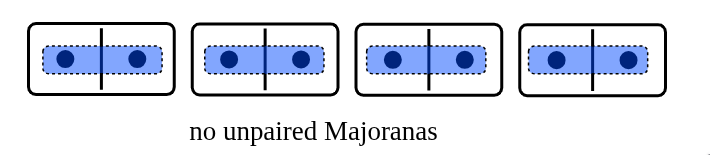
\includegraphics[width=0.45\textwidth]{../External_Figs/no_unpaired.png}
  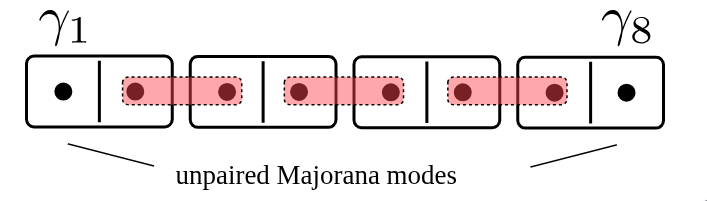
\includegraphics[width=0.45\textwidth]{../External_Figs/unpaired.png}
  \caption{Schematic representation of the Kitaev chain in its two distinct phases. Left: In the trivial phase, Majorana modes on the same site pair to form conventional fermions, leaving no unpaired modes. Right: In the topological phase, Majoranas on adjacent sites couple, leaving unpaired modes at the chain ends, which combine into a non-local fermionic mode. \textcolor{red}{CITATION}Topocondmat.org (Bulk edge correspondence in Kitaev chains)}
  \label{fig:kitaev}
\end{figure}
In the figure above \ref{fig:kitaev}, we see a schematic representation of the Kitaev chain in its two distinct phases, the trivial phase on the left and the topological phase on the right.\\
In the trivial phase, the Majorana modes on the same site pair to form conventional fermions, leaving no unpaired modes. In contrast, in the topological phase, Majoranas on adjacent sites couple, leaving unpaired modes at the chain ends, which combine into a non-local fermionic mode. At first glance, it may seem impossible to isolate a single Majorana mode, since condensed matter systems are composed of electrons, which always correspond to pairs of Majoranas. However, it turns out that by engineering the Hamiltonian appropriately, one can create a situation where two Majorana modes localize at opposite ends of a one-dimensional system, effectively separating them spatially. This separation is crucial for their non-Abelian statistics and potential applications in topological quantum computing\textcolor{red}{CITATION}[Topocondmat].\\
The Hamiltonian of the Kitaev chain is given by:
\begin{equation}
H = -\mu \sum_{j=1}^{N} \left(c_j^\dagger c_j - \frac{1}{2}\right)
- t \sum_{j=1}^{N-1} \left(c_j^\dagger c_{j+1} + c_{j+1}^\dagger c_j\right)
+ \Delta \sum_{j=1}^{N-1} \left(c_j c_{j+1} + c_{j+1}^\dagger c_j^\dagger\right),
\label{eq:kitaev_ham}
\end{equation}
where $μ$ is the chemical potential, or onsite energy, $t$ is the hopping amplitude, and $Δ$ is the p-wave pairing amplitude. The fermionic operators $c_j^\dagger$ and $c_j$ create and annihilate an electron at site $j$, respectively.\\
With the parameters $t=Δ=0$ and $μ ≠ 0$, the system is in a trivial insulating phase with no special edge states. However, tuning the parameters such that $t = Δ > 0$ and $μ = 0$, the edges become isolated, leaving two unpaired Majorana modes localized at the ends. These modes combine into a single non-local fermionic mode that costs zero energy to occupy. We will later explore how this model maps onto the QD–SC–QD system, and how the parameters can be tuned experimentally to reach this regime. 


\subsubsection{Bulk spectrum and topological phases}
To understand when the Kitaev chain supports topologically non-trivial states, we now turn from the real-space picture to its bulk description in momentum space. This transformation allows us to analyze the quasiparticle excitation spectrum and identify the conditions under which the superconducting gap closes and reopens.\\
Using translation invariance, we apply a Fourier transform,
$$
c_j = \frac{1}{\sqrt{N}} \sum_p e^{ipaj} c_p,
$$
This allows us to write the Hamiltonian (\ref{eq:kitaev_ham}) in momentum space $p$ as:
\begin{equation}
H = ∑_{ p}^{} ξ_p\left(c_p^{†} c_p - \frac{1}{2}\right) - ∑_{p}^{} t \cos p a + Δ ∑_{p}^{}\left(c_p^{†} c_{-p}^{†} e^{ipa} + c_{-p} c_p e^{-ipa}\right), 
\end{equation}
with $ξ_p = -μ - 2t \cos pa$ and $a$ the lattice spacing. This Hamiltonian becomes diagonal in the Bogoliubov–de Gennes (BdG) formalism. The resulting quasiparticle energy spectrum is:
\begin{equation}
  E_{p,\pm} = \pm \sqrt{(μ - 2t \cos{pa})^2 + 4Δ^2 \sin^2{pa}},
\end{equation}
The spectrum is gapped for most parameter values, but the gap closes when
$$
|μ| = 2|t|
$$
This marks the critical point separating two distinct superconducting phases. When $μ$ crosses this boundary, the system undergoes a topological phase transition: the character of the ground state changes without any symmetry breaking, but through a change in the topology of the quasiparticle band structure.\\
\begin{figure}
  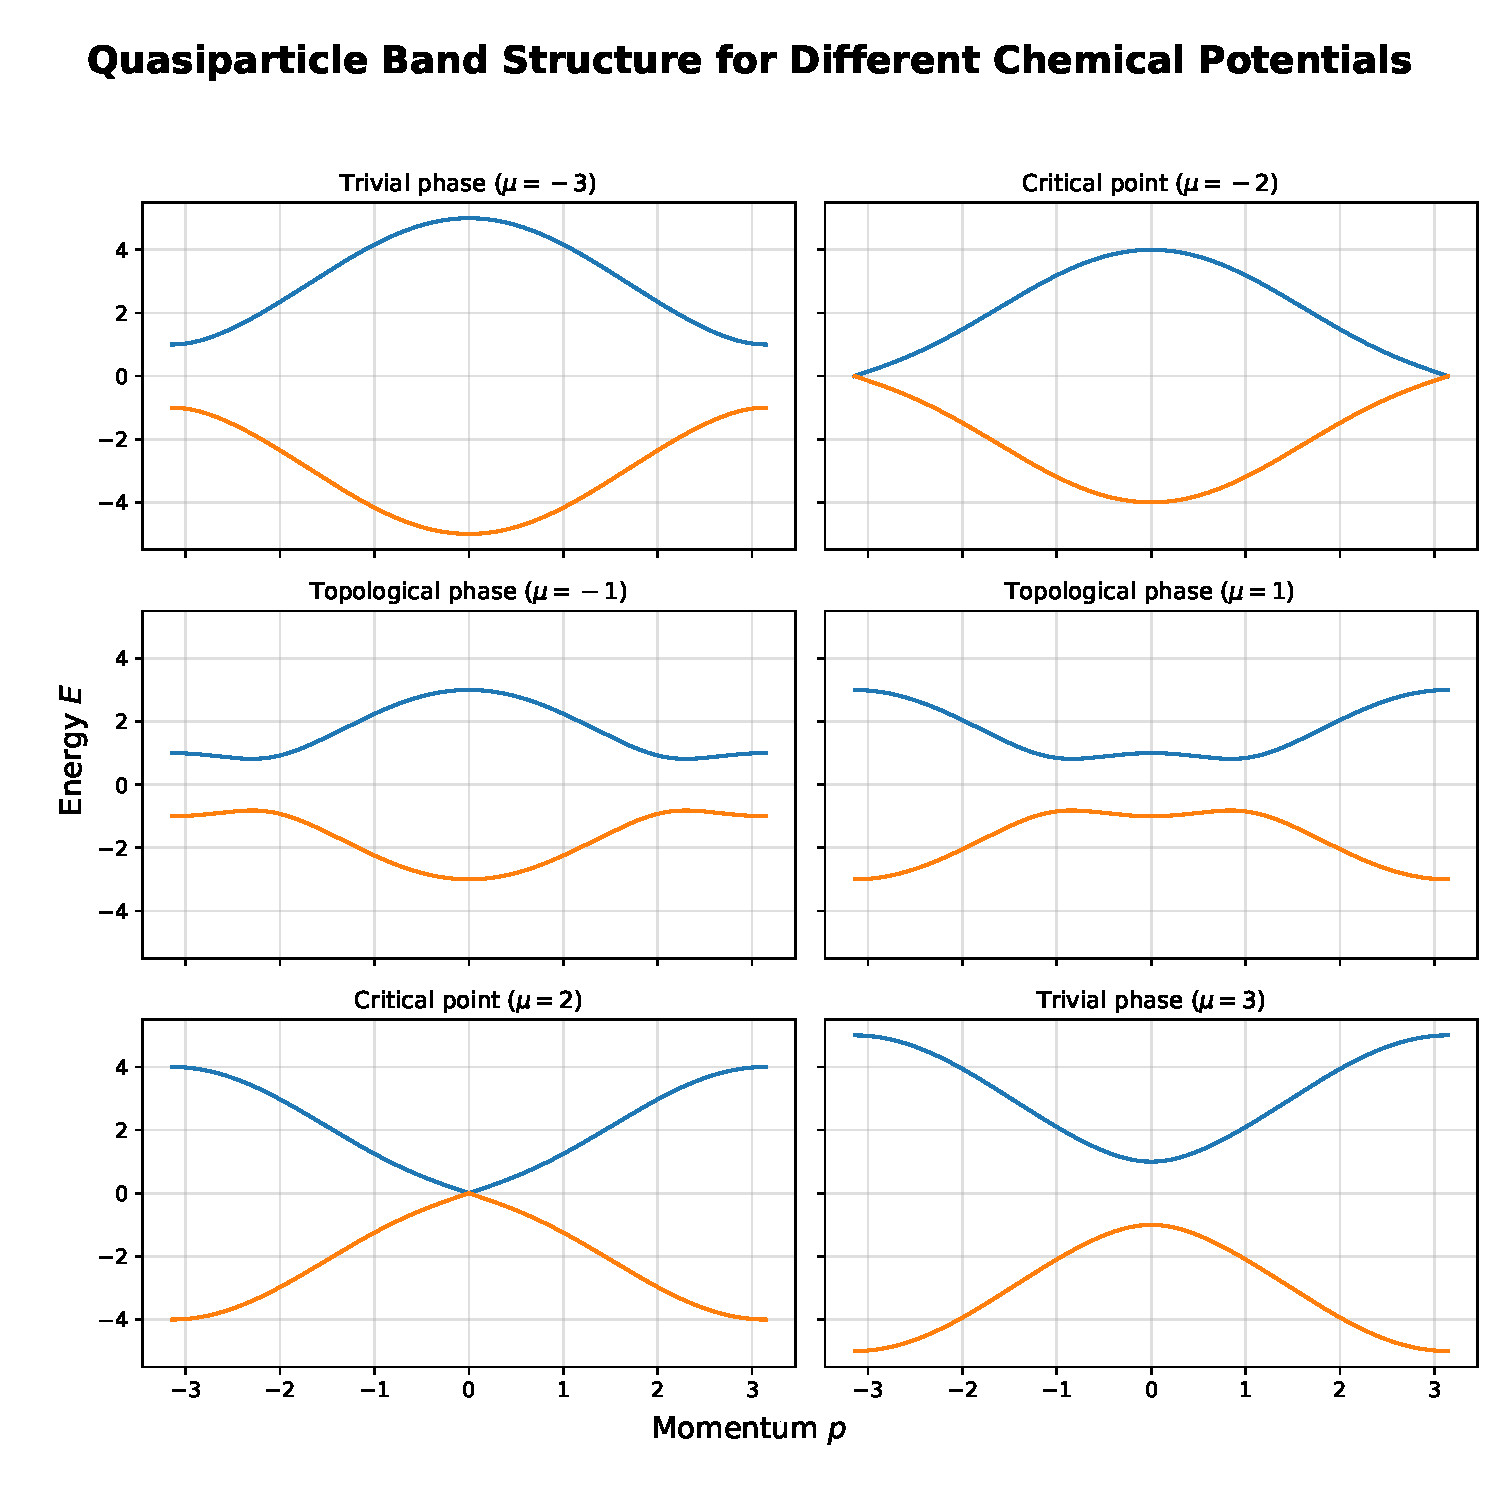
\includegraphics[width=1\textwidth]{../Figures/band_structure.pdf}
  \caption{Quasiparticle energy spectrum of the Kitaev chain for different chemical potentials $μ$. Left: In the trivial phase ($|μ| > 2|t|$), the spectrum is fully gapped with no zero-energy modes. Right: In the topological phase ($|μ| < 2|t|$), the gap closes and reopens, signaling the emergence of zero-energy edge modes.}
\end{figure}
\newpage


\subsubsection{Majorana representation and zero modes}
In order to further understand the nature of these boundry states, we can express each fermionic operator in terms of two real Majorana operators:
\begin{equation}
c_j = \frac{1}{2}(\gamma_j^A + i\gamma_j^B), \quad
c_j^\dagger = \frac{1}{2}(\gamma_j^A - i\gamma_j^B),
\end{equation}
where $\gamma_j^{A,B}$ satisfy $\{\gamma_j^\alpha, \gamma_k^\beta\} = 2\delta_{jk}\delta_{\alpha\beta}$ and $(\gamma_j^\alpha)^\dagger = \gamma_j^\alpha$.\\
In this basis, the two distinct phases correspond to different pairing patterns between the Majorana operators. For a large $μ$, ($|μ| > 2|t|$), the Majorana operators pair up on the same site, leading to a trivial phase with no zero-energy modes. On the other hand, in the topological phase ($|μ| < 2|t|$) and $t = Δ$, the Majoranas on adjacent sites couple ($\gamma_j^B$ with $\gamma_{j+1}^A$), leaving two unpaired Majorana modes at the ends of the chain: $\gamma_1^A$ at the left end and $\gamma_N^B$ at the right end.\\
These two unpaired Majoranas combine into a single non-local fermionic mode:
\begin{equation}
  f = \frac{1}{2 }(\gamma_1^A + i\gamma_N^B),
\end{equation}
which satisfies $\{f, f^\dagger\} = 1$ and costs zero energy. The two possible occupations of this non-local fermion correspond to a twofold degenerate ground state. This degeneracy is topologically protected: local perturbations cannot lift it unless they close the bulk gap or couple the two edge Majoranas directly.\\
The Kitaev chain thus provides the minimal theoretical framework for understanding Majorana zero modes. Its simplicity allows for exact solutions and clear physical intuition, making it an ideal starting point for exploring more complex systems that can host topological superconductivity and Majorana fermions.

\subsection{The QD–SC–QD System as an Effective Kitaev Chain}
While the Kitaev chain provides the minimal theoretical framework for understanding Majorana zero modes, it remains an abstract model, assuming spinless fermions and idealized $p$-wave pairing. Real materials, however, are spinful and typically host conventional $s$-wave superconductivity. The challenge, therefore, is to engineer hybrid systems whose effective low-energy behaviour mimics that of the Kitaev chain.\\
A particularly compact realization of such a system is the double quantum dot coupled via a superconducting segment, the so-called \textit{Poor Man’s Majorana} (PMM) setup. This device consists of two quantum dots (QDs) connected through a central superconductor, forming the minimal two-site analogue of the Kitaev chain. Despite its simplicity, it reproduces the essential ingredients of topological superconductivity: coherent hopping, non-local pairing, and the emergence of near-zero-energy states with Majorana-like characteristics.
\subsubsection{Mapping to the Kitaev Hamiltonian}

Each quantum dot represents a site in the minimal Kitaev chain. The Hamiltonian of the hybrid system can be written in a general form as:
\begin{equation}
H = \sum_{i=L,R} \epsilon_i n_i
+ t (d_L^\dagger d_R + d_R^\dagger d_L)
+ \Delta (d_L^\dagger d_R^\dagger + d_R d_L)
+ U \sum_{i=L,R} n_i
\label{eq:qdsqdh}
\end{equation}
where $d_{L/R}^\dagger$ and $d_{L/R}$ are electron creation and annihilation operators on the left and right dots. $n_i$ is the number operator for dot $i$. The parameters $ϵ_{L,R}$ correspond to the dot energy levels, $t$ is the elastic cotunneling amplitude, $Δ$ is the crossed Andreev reflection amplitude, and $U$ is the on-site Coulomb repulsion energy.\\
The meaning of each parameter is as follows:
\begin{itemize}
    \item \textbf{Elastic cotunneling (ECT):} An electron tunnels coherently from one dot to the other via a virtual process through the superconductor. This process defines the effective hopping amplitude $t$, analogous to the kinetic term in the Kitaev model.
    \item \textbf{Crossed Andreev reflection (CAR):} A Cooper pair in the superconductor splits such that one electron tunnels into each dot. This process produces an effective non-local pairing term $\Delta$, which is mathematically equivalent to the $p$-wave pairing amplitude in the Kitaev chain.
    \item \textbf{On-site energy:} The local dot energies $\epsilon_L$ and $\epsilon_R$ play the role of the site-dependent chemical potential $\mu$.
\end{itemize}
At the so-called sweet spot, where $|\epsilon_L| = |\epsilon_R| = 0$ and $|t| = |\Delta|$, the system enters a regime in which two Majorana-like states localize predominantly on separate dots. These two states form an effective non-local fermion and exhibit many of the qualitative features of true topological Majorana bound states, such as zero-energy modes and near-perfect particle–hole symmetry. However, since the system is finite and lacks a bulk, it does not possess true topological protection, hence the name “poor man’s Majoranas.”

\subsubsection{Low-energy features and experimental tunability}
The poor man's Majorana setup, double quantum dot coupled via a superconductor, provides a minimal realization of the Kitaev chain. In reality, the complete microscopic Hamiltonian includes interactions and spin degrees of freedom. However, in the regime relevant for Poor Man's Majoranas, the low-energy physics is effectively captured by the spinless two-site model introduced above. In this setup, near-zero energy Majorana-like states emerge across the two dots, exhibiting an even- and odd-parity ground state and strong non-local correlations.\\
This platform is an experimentally attractive method to realize Kitaev chain physics because its parameters can be tuned independently. Gate voltages control the dot energy levels, the transparency of the QD–SC interfaces governs the effective hopping and non-local pairing, and magnetic fields can suppress unwanted spinful excitations. By sweeping these parameters, one can access and identify the  Majorana-like properties. \\
This minimal setup captures the essential low-energy properties of a Kitaev chain while remaining experimentally controllable, providing a direct route from theoretical modeling to realizable quantum devices.
\subsection{Identifying Majorana Modes in the QD–SC–QD System}\label{sec:IdentifyingMajoranaModes}
In this section we will briefly go through the key signatures that indicate the presence of Majorana-like modes in the QD–SC–QD system. These signatures arise from the unique properties of Majorana fermions. There are a few metrics we can use to identify the presence of PMMs, and their rigidity to perturbations.\\
\subsubsection{The parity operator}
The parity operator itself is not a measurement of a Majorana mode, but it is a useful tool in the identification process. The mean-field Hamiltonian of a superconductor does not conserve particle number, but it does conserve fermion parity. What this means is that the number of electrons in the system can change by pairs, but not by single electrons. The parity operator is defined as:
$$
P = (-1)^{N} = 1 - 2c_n ^{†} c_n
$$
where $N$ is the total number of electrons in the system, and $c_n^{†}$ and $c_n$ are the creation and annihilation operators for the fermionic mode formed by the two Majorana modes. The eigenvalues of the parity operator are $+1$ for even parity (an even number of electrons) and $-1$ for odd parity (an odd number of electrons).\\
When working with Majorana modes, we often consider the two degenerate ground states of the system, which differ by their fermion parity. The presence of a Majorana mode implies that these two states are nearly degenerate and can be transformed into each other by adding or removing a single electron, thus changing the parity.\\

\subsubsection{Energy degeneracy}
When we try to identify Majorana modes in the QD–SC–QD system, one of the primary signatures we look for is the presence of energy degeneracy between the even and odd parity ground states. We also want the ground state energies to be separeted by a finite energy gap from the excited states. This energy gap protects the Majorana modes from local perturbations and thermal excitations, which is crucial for their stability and potential use in quantum computing. This is because when we want to do quantum computation using Majorana modes, we need to be able to manipulate the states without causing transitions to higher energy states.\\
\begin{figure}
  \centering
  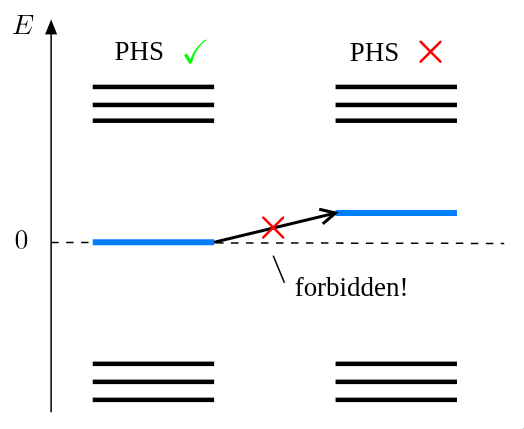
\includegraphics[width=0.5\textwidth]{../External_Figs/gs_symmetry.png}%
  \caption{Energy spectrum showing how the energy eigenvalues of the system must be symmetric around zero energy due to particle-hole symmetry \textcolor{red}{CITATION}Topocondmat.org (Bulk edge correspondence in Kitaev chains)}
  \label{fig:gs_symmetry}
\end{figure}
\newpage
\subsubsection{Local distinguishability}
A property of the Kitaev chain in its topological phase is that measurements done locally cannot reveal if the system is in its odd or even ground state. Meaning the two ground states are locally indistinguishable. In order to quantify this property, we will define the local distinguishability parameter LD as:
$$
\text{LD} = \frac{1}{N} \sum_{j=1}^{N} || ρ_j^o - ρ_j^e || = \frac{1}{N} \sum_{j=1}^{N} || δ ρ_j ||
$$
\textcolor{red}{CITATION}[Majorana bound states in chains
of interacting quantum dots Viktor ].\\Here, $ρ_j^{o/e}$ are the reduced density matrices of site $j$ for the odd and even parity ground states, respectively. The norm $|| \cdot ||$ is the trace norm, which measures the difference between the two local states. The LD parameter quantifies how distinguishable the two ground states are when only local measurements are considered. A value of LD close to zero indicates that the two states are nearly indistinguishable locally, which is a hallmark of Majorana modes. Conversely, a value close to one indicates that the states can be easily distinguished by local measurements, suggesting the absence of Majorana modes.\\
\subsubsection{Majorana polarization}
In interaction Kitaev chains with finite magnetic fields, there are no ideal Majorana sweet spots, as the presence of the other spin species introduces corrections to the simple picture of Majorana modes. However, sweet spots with very good Majorana localization and close to degenerate ground states with even and odd parity can still appear in the system. To quantify how close we are to an ideal Majorana mode, we can use the Majorana polarization (MP) metric. The MP is a measure of how well the Majorana modes are localized at the ends of the chain and how closely they resemble ideal Majorana fermions. The MP is defined as:
$$
M_α = \frac{W_α^2 - Z_α^2}{W_α^2 + Z_α^2}
$$
where,
$$
W_α = ∑_{σ} \bra{o} c_{ασ} + c_{ασ}^{†} \ket{e}, \quad Z_α = i ∑_{σ} \bra{o} c_{ασ} - c_{ασ}^{†} \ket{e}
$$
Here, $α$ denotes the site index (left or right dot), $σ$ is the spin index, and $\ket{o}$ and $\ket{e}$ are the odd and even parity ground states, respectively. In an ideal sweet spot where two Majoranas are perfectly localized on the left and right dots, the MP values would be $M_L = -M_R = ± 1$. \textcolor{red}{CITATION}[Chap3 qtech].\\
\subsubsection{Charge expectation and non-locality}
The last measurable property we will discuss is the charge expectation value of the ground states. This id measured by taking the expectation values of the number operators in the odd and even ground states:
$$
\bra{e}n_{L(R)} \ket{e}, \quad \bra{o}n_{L(R)} \ket{o}
$$
where $n_{L(R)}$ is the number operator for the left (right) dot. In the ideal case, these expectation values should be equal for both ground states. This is because, if the difference is zero, the two ground states share the same local charge distribution, making them locally indistinguishable. 




















\section{Analytical and Numerical Investigation of PMMs}
Present my work and demonstrate how to apply theory to a concrete problem.\par
\subsection{Single particle model:}
% \subsubsection{The Model Hamiltonian:} Present the minimal Hamiltonian for the QD-SC-QD system that i have in my notes note section 5.2.2, for instance Eq 3.54 from chap3.pdf. Define all the terms clearly. This will be the Hamiltonian I use.\par
% $$  
%   H = \begin{pmatrix}
%     ϵ_L & t & 0 & Δ \\
%     t & ϵ_R & -Δ & 0 \\
%     0 & -Δ & -ϵ_L & -t \\
%     Δ & 0 & -t & -ϵ_R
%   \end{pmatrix}
% $$
% Where $ϵ_L$ and $ϵ_R$ are the energy levels of the left and right dots, $t$ is the elastic cotunneling amplitude, and $Δ$ is the CAR amplitude. The basis is $(d_L, d_R, d_L^{†}, d_R^{†})$, called the Nambu basis. The operators $d_L^{†}$ and $d_R^{†}$ create an electron in the left and right dot, respectively.\par
\subsubsection{The Model Hamiltonian}

The minimal Hamiltonian describing the QD–SC–QD system is given in the Nambu basis $\Psi^\dagger = (d_L, d_R, d_L^\dagger, d_R^\dagger)$ as

\begin{equation}
  H = \begin{pmatrix}
    \epsilon_L & t & 0 & \Delta \\
    t & \epsilon_R & -\Delta & 0 \\
    0 & -\Delta & -\epsilon_L & -t \\
    \Delta & 0 & -t & -\epsilon_R
  \end{pmatrix},
\end{equation}

where $\epsilon_L$ and $\epsilon_R$ denote the energy levels of the left and right quantum dots, $t$ is the elastic cotunneling amplitude between dots, and $\Delta$ is the crossed Andreev reflection (CAR) amplitude induced by the central superconductor. The operators $d_L^\dagger$ and $d_R^\dagger$ create an electron on the left and right dot, respectively. This 4×4 Hamiltonian captures the essential low-energy physics of the two-dot system in the spinless approximation.

\subsubsection{Analytical determination of the sweet spot}
To identify the condition for zero-energy Majorana modes, we first consider the simplest case of two identical quantum dots with energy levels at zero, \(\epsilon_L = \epsilon_R = 0\). Solving the eigenvalue problem \(H \Psi = E \Psi\) leads to the characteristic polynomial:
\[
\det(H - E I) = E^4 - E^2 a + b = 0,
\]
where
\[
a = \epsilon_L^2 + \epsilon_R^2 + 2(t^2 + \Delta^2), \quad
b = (t^2 - \epsilon_L \epsilon_R - \Delta^2)^2.
\]
The solutions for \(E^2\) are
\[
E^2 = \frac{a \pm \sqrt{a^2 - 4b}}{2}.
\]
The discriminant simplifies to 
\[
a^2 - 4b = \big[(\epsilon_L + \epsilon_R)^2 + 4t^2\big] \big[(\epsilon_L - \epsilon_R)^2 + 4\Delta^2\big].
\]
For zero-energy solutions (\(E = 0\)), we require \(b = 0\), which gives
\[
t^2 - \epsilon_L \epsilon_R - \Delta^2 = 0.
\]
At \(\epsilon_L = \epsilon_R = 0\), this reduces to the sweet spot condition:
\[
|t| = |\Delta|.
\]
Under this condition, the four eigenvalues of the Hamiltonian are
\[
E = \{0, 0, +2|t|, -2|t|\}.
\]
Thus, two zero-energy modes appear, while the remaining two states are finite-energy excitations separated by a gap \(2|t|\).

\subsubsection{Zero-mode eigenvectors and physical interpretation}
The eigenvectors corresponding to the zero-energy modes are
\[
v_1 = \begin{pmatrix} 1 \\ 0 \\ 1 \\ 0 \end{pmatrix}, \quad
v_2 = \begin{pmatrix} 0 \\ 1 \\ 0 \\ -1 \end{pmatrix},
\]
which in operator form correspond to self-conjugate Majorana operators:
\[
\gamma_1 \propto d_L + d_L^\dagger, \quad
\gamma_2 \propto d_R - d_R^\dagger.
\]
These states are spatially separated, with \(\gamma_1\) localized on the left dot and \(\gamma_2\) on the right dot. They satisfy the Majorana condition \(\gamma = \gamma^\dagger\) and form the Poor Man's Majorana modes of the system. Their degeneracy encodes the nonlocal fermionic parity, which is the key resource for quantum information applications.
The finite-energy eigenvectors,
\[
v_3 \propto \begin{pmatrix}-1 \\ 1 \\ 1 \\ 1\end{pmatrix}, \quad
v_4 \propto \begin{pmatrix}1 \\ 1 \\ -1 \\ 1\end{pmatrix}, \quad
E = \pm 2|t|,
\]
are delocalized Bogoliubov quasiparticles. These define the energy gap protecting the zero-mode subspace. As long as this gap remains finite, the Majorana modes remain robust against small perturbations and do not hybridize with the higher-energy states.
The analytical solution confirms that the sweet spot for zero-energy Majoranas occurs at \(|t| = |\Delta|\) with dot energies set to zero, and the corresponding eigenvectors clearly illustrate the spatial separation and particle–hole symmetry characteristic of Majorana modes.

% \subsubsection{Numerical Simulations - Visualize the Emergence of Majoranas:} Build and diagonalize the Hamiltonian numerically. Band Structure: Plot the two lowest positive energy eigenvalues as a function of a dot's energy $ϵ_L$ (keeping $ϵ_R = 0$) and $t = Δ$. Reproduce the plot from Fig 3.5a in chap3.pdf showing two states remaining at zero energy, showcasing the symmetry. Wavefunctions: At the sweet spot ($t = Δ$ and $ϵ_L = ϵ_R = 0$), find the eigenvectors for the two zero-mode energy states. Plot the magnitude of the components. I should be able to see that one zero mode is localized entirely on the left dot and the other is entirely on the right dot, confirming they are spatially separated Majoranas.\par
% \subsubsection{Numerical Work - Probing Protection and Robustness:} Detuning $t$ and $Δ$: Vary $t$ and $Δ$ away from the sweet spot. Plot the lowest energy eigenvalue as I varyt he ratio $\frac{t}{Δ}$ away from 1. This will show that the zero-energy states immediately split and acquire a finite energy gap, demonstrating their lack of full topological protection. Detuning Dot Energies: Vary $ϵ_L$ and $ϵ_R$ away from zero while keeping $t = Δ$. The degeneracy should be lifted quadratically. My results here should quantify the robustness of the PMMs to local perturbations. I can conclude that while they are not fully protected like in a true topological system, the degeneracy is protected against certain local perturbations to first order.\par
\subsubsection{Numerical Simulations – Visualizing the Emergence of Majoranas}

To confirm the analytical predictions and illustrate the emergence of Majorana-like states, we diagonalized the spinless two-site Hamiltonian numerically.

\begin{figure}[htbp]
  \centering
  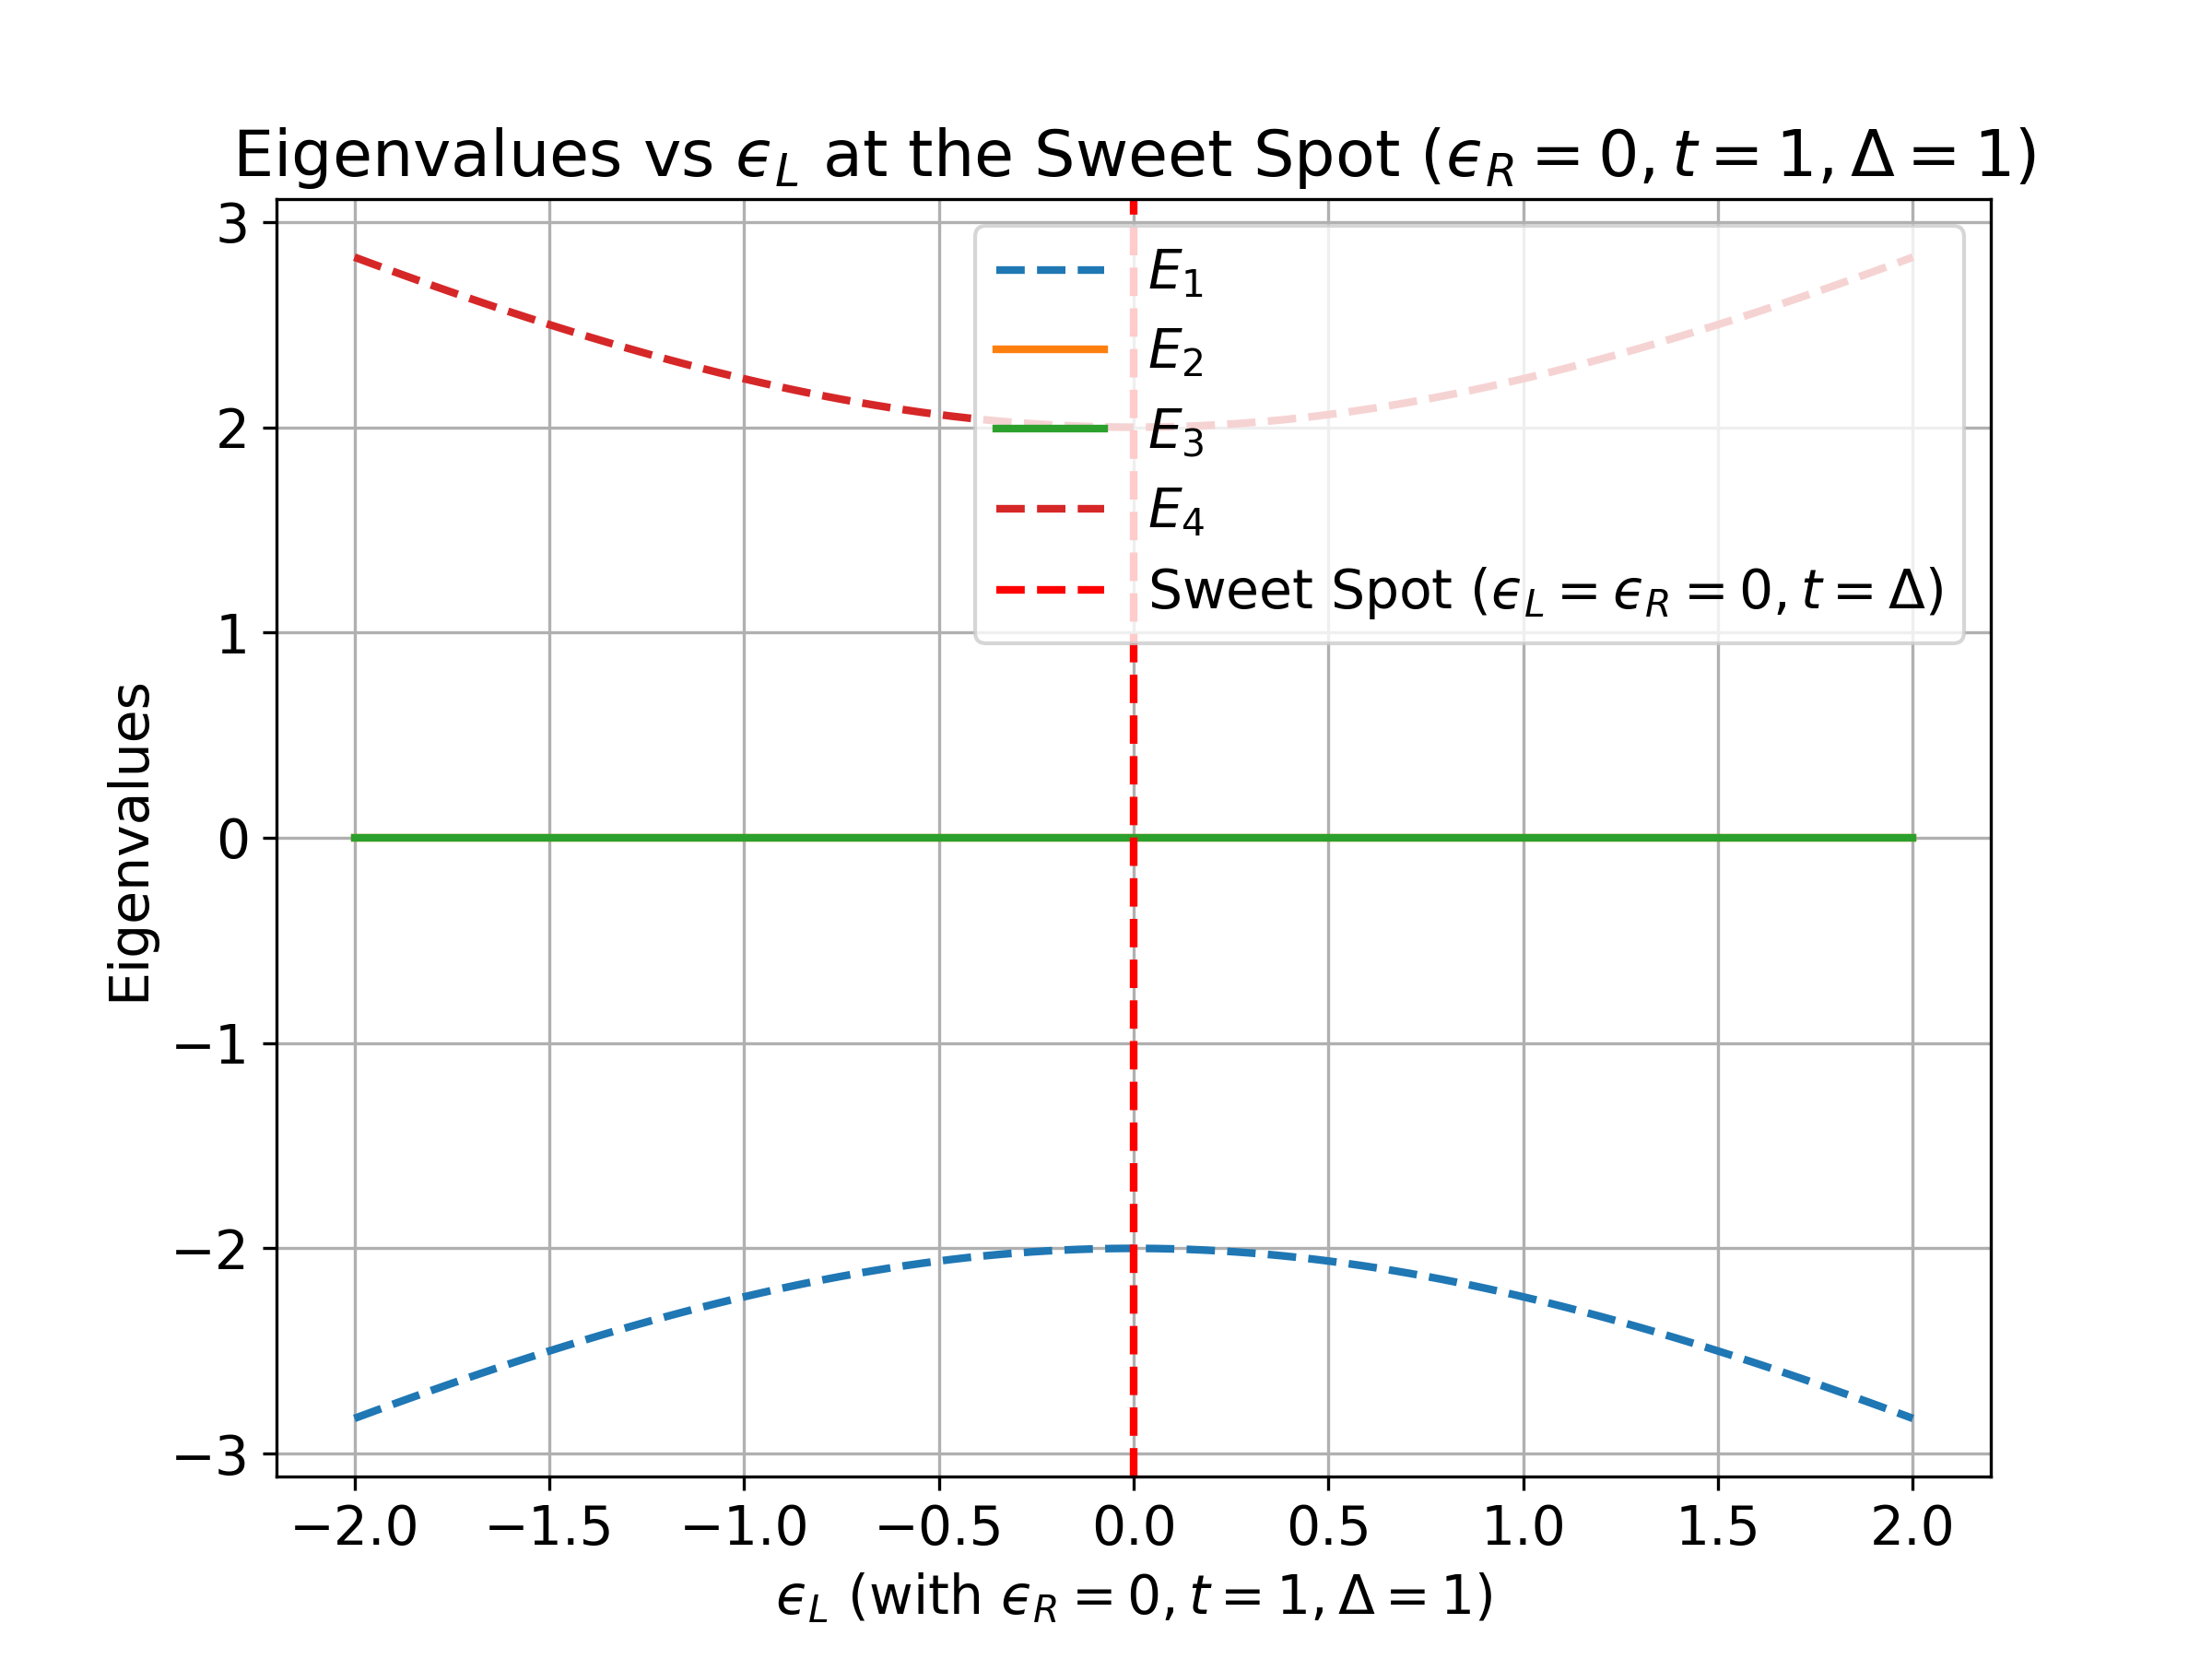
\includegraphics[width=0.7\textwidth]{../Figures/singlebody_sweetspot_eps.png}
  \caption{(a) Lowest energy eigenvalues as a function of $\epsilon_L$ with $\epsilon_R = 0$ and $t = \Delta$. Two states remain pinned at zero energy, forming Majorana-like zero modes.}
  \label{fig:sb_epsL}
\end{figure}

\begin{figure}[htbp]
  \centering
  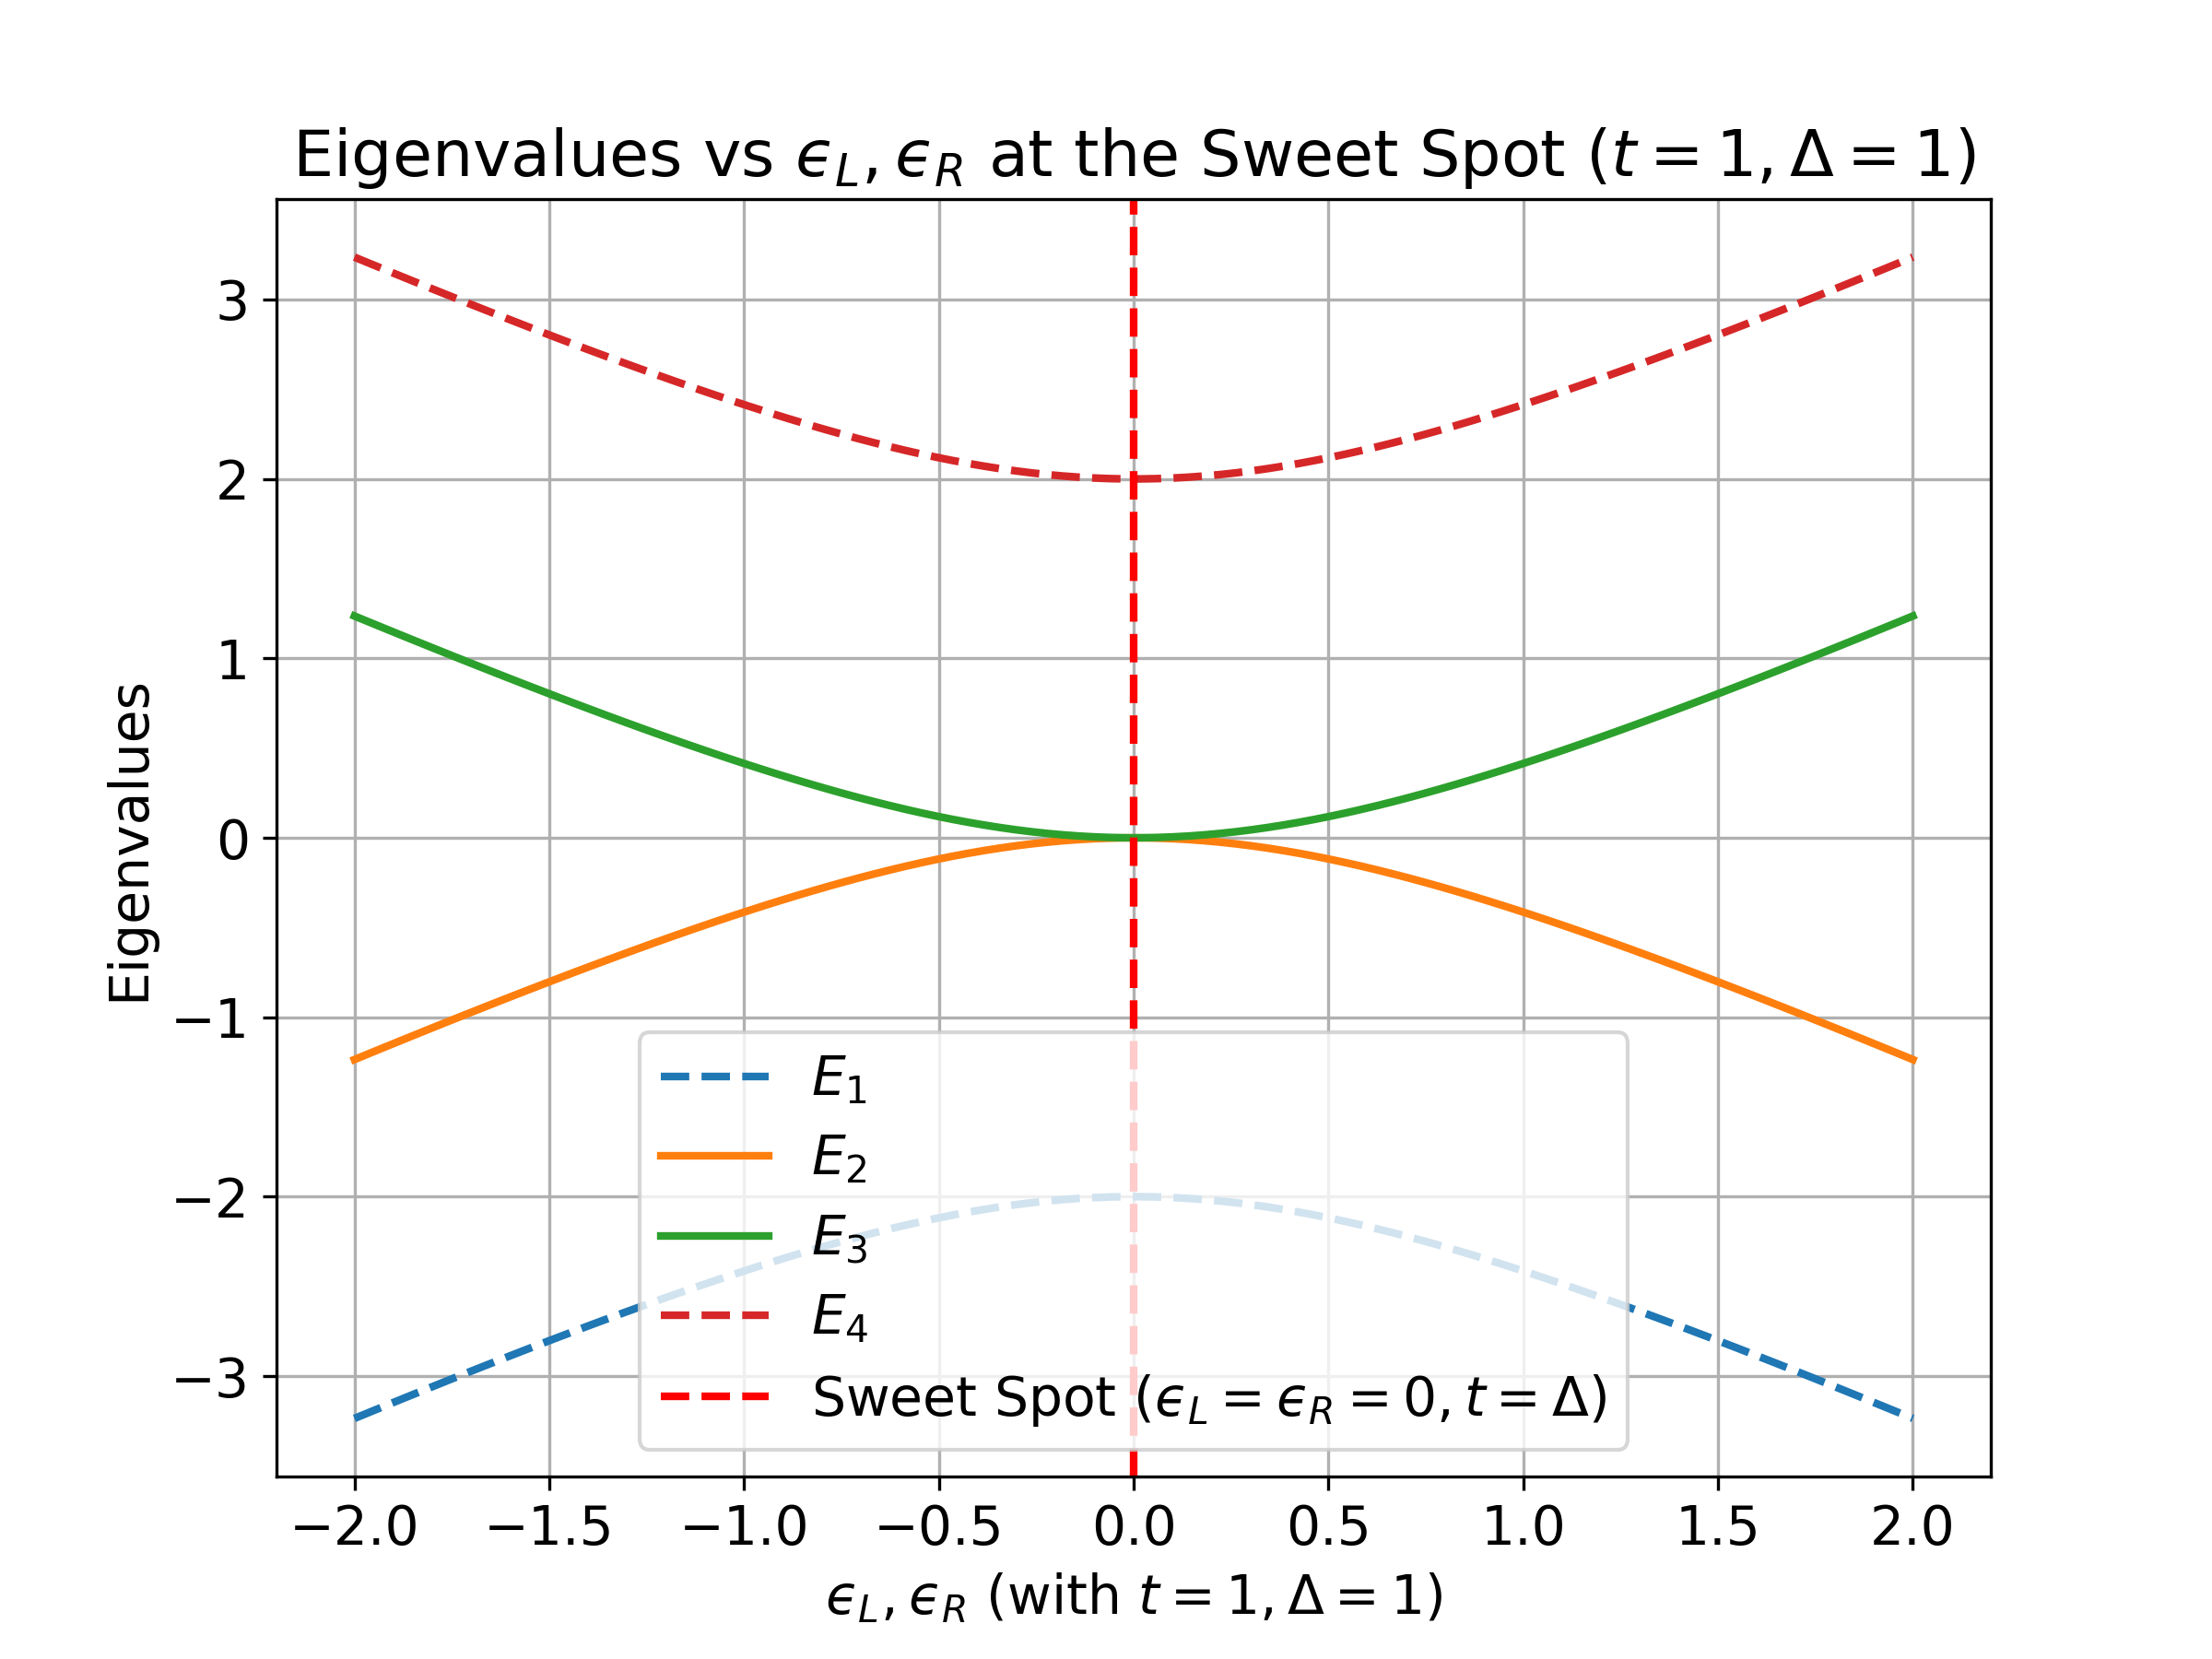
\includegraphics[width=0.7\textwidth]{../Figures/singlebody_sweetspot_epsLR.png}
  \caption{(b) Eigenvalues as both $\epsilon_L$ and $\epsilon_R$ are varied around zero, showing the preservation of zero-energy modes at the sweet spot, and their splitting away from it.}
  \label{fig:sb_epsLR}
\end{figure}

\begin{figure}[htbp]
  \centering
  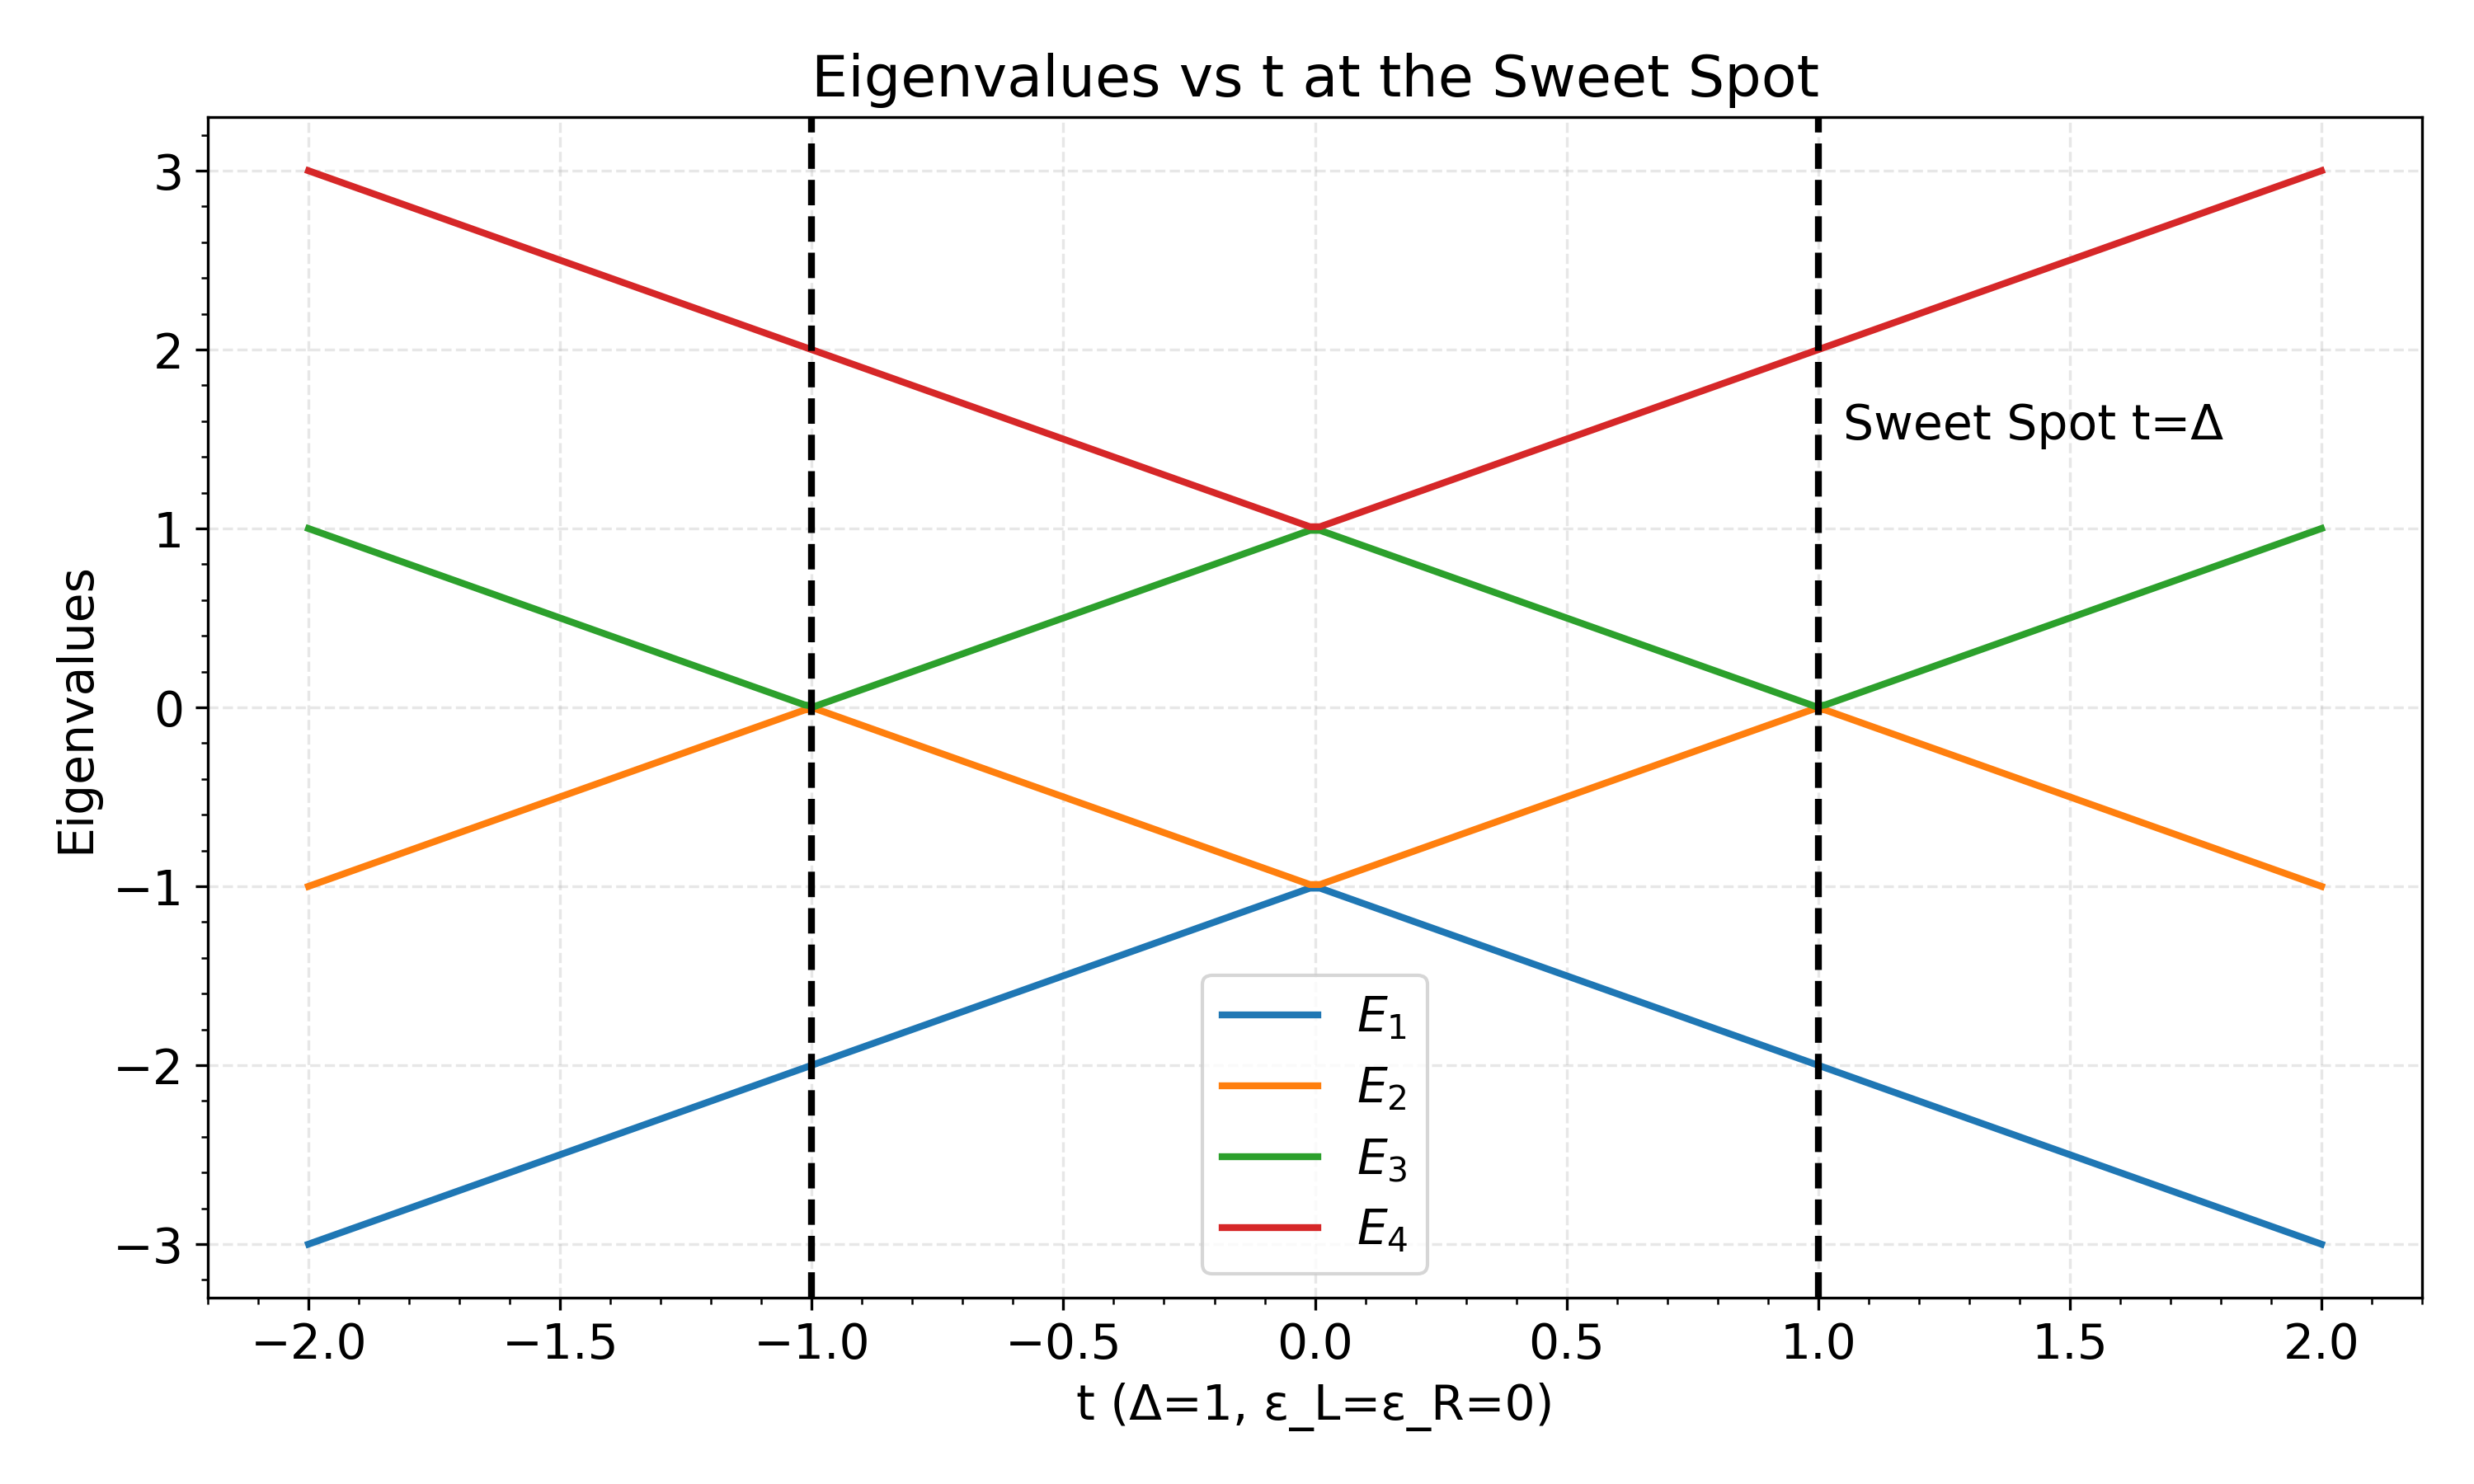
\includegraphics[width=0.7\textwidth]{../Figures/singlebody_sweetspot_t.png}
  \caption{(c) Zero-mode energies versus hopping $t$ at $\Delta = 1$, $\epsilon_L = \epsilon_R = 0$, demonstrating that degeneracy is maintained only at $t = \Delta$.}
  \label{fig:sb_tscan}
\end{figure}
\newpage
Figure ~\ref{fig:sb_epsL}, ~\ref{fig:sb_epsLR}, and ~\ref{fig:sb_tscan} show how we diverge from the sweet spot by varying $\epsilon_L$, $\epsilon_R$, and $t$, away from our analyrical sweet spots.\\
At the sweet spot ($\epsilon_L = \epsilon_R = 0$, $t = \Delta$), the eigenvectors corresponding to the zero-energy states are extracted. Figure~\ref{fig:sb_zero_modes} shows the magnitude of their components in the Nambu basis $(d_L, d_R, d_L^\dagger, d_R^\dagger)$. One zero mode is localized entirely on the left dot, and the other on the right dot, confirming the spatial separation characteristic of Majorana modes.

\begin{figure}[htbp]
  \centering
  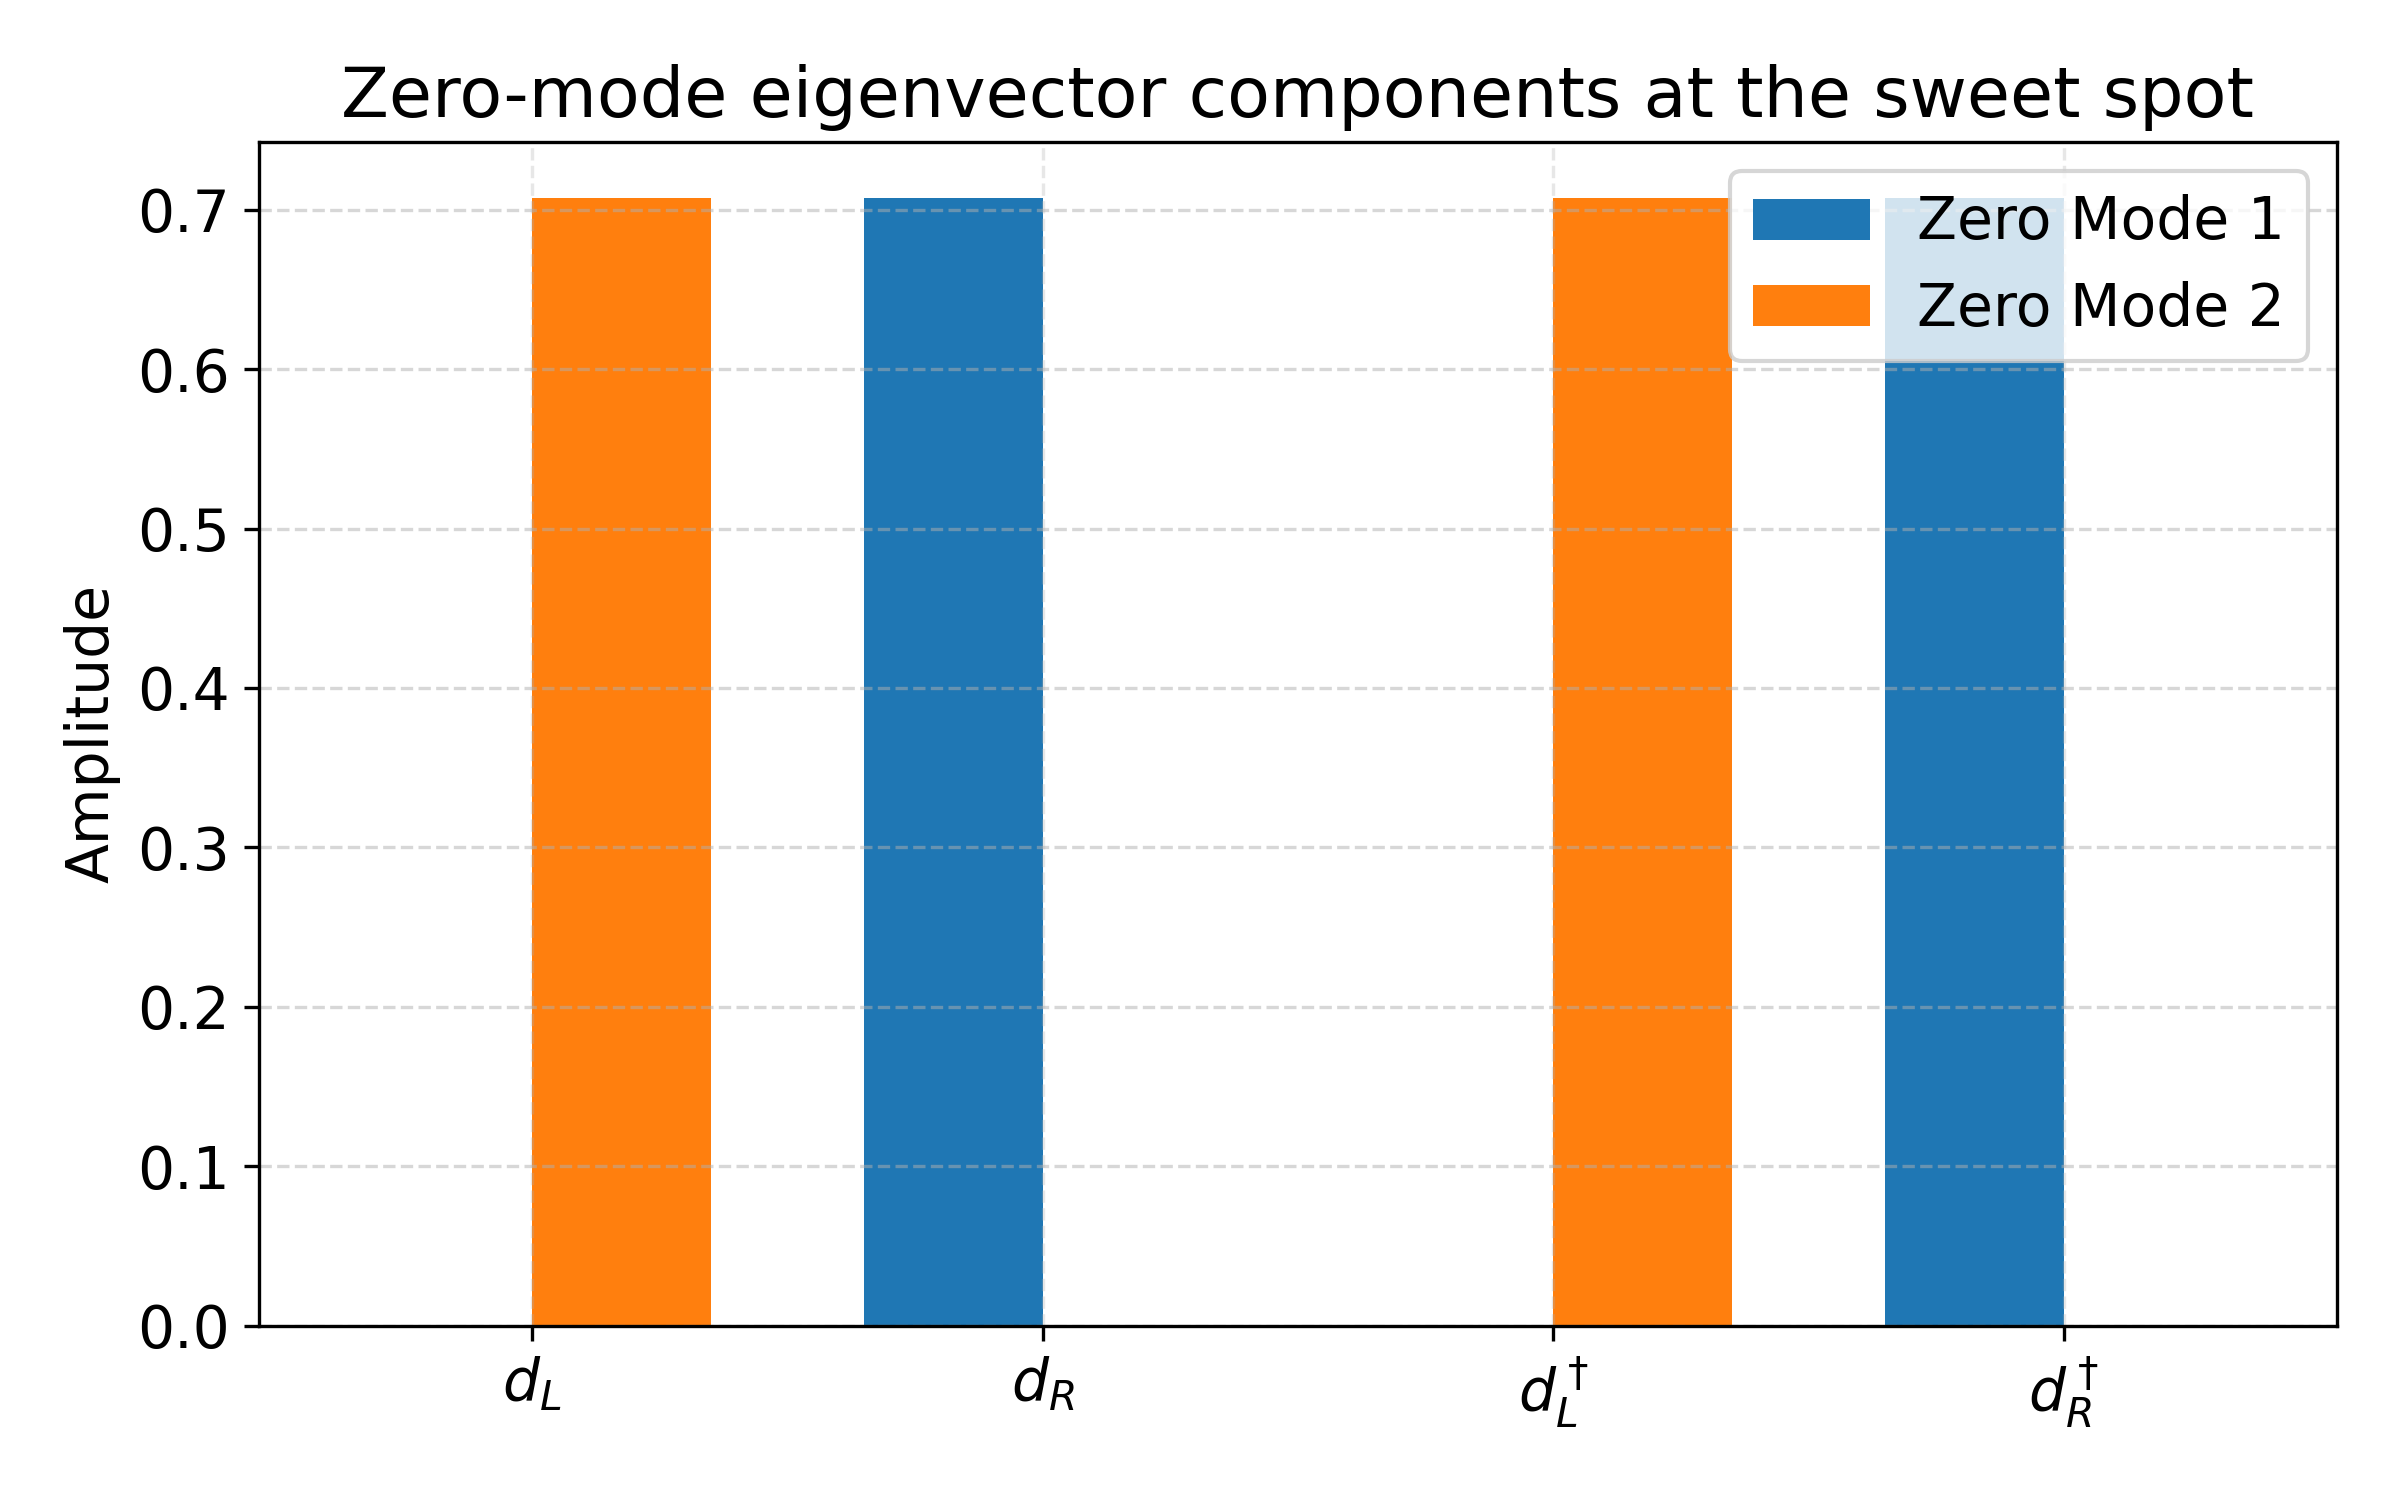
\includegraphics[width=0.7\textwidth]{../Figures/singlebody_sweetspot_zero_modes.png}
  \caption{Component amplitudes of the zero-energy eigenvectors at the sweet spot. Spatial separation of the modes confirms the Majorana character.}
  \label{fig:sb_zero_modes}
\end{figure}

\subsubsection{Numerical Work – Probing Protection and Robustness}

To probe the stability of the zero modes, we vary system parameters away from the sweet spot. Figure~\ref{fig:sb_grid} presents a contour map of the lowest energy splitting versus $t$ and $\Delta$ at $\epsilon_L = \epsilon_R = 0$. Deviations from $t = \Delta$ immediately lift the degeneracy, showing that the zero modes are not fully topologically protected.

\begin{figure}[htbp]
  \centering
  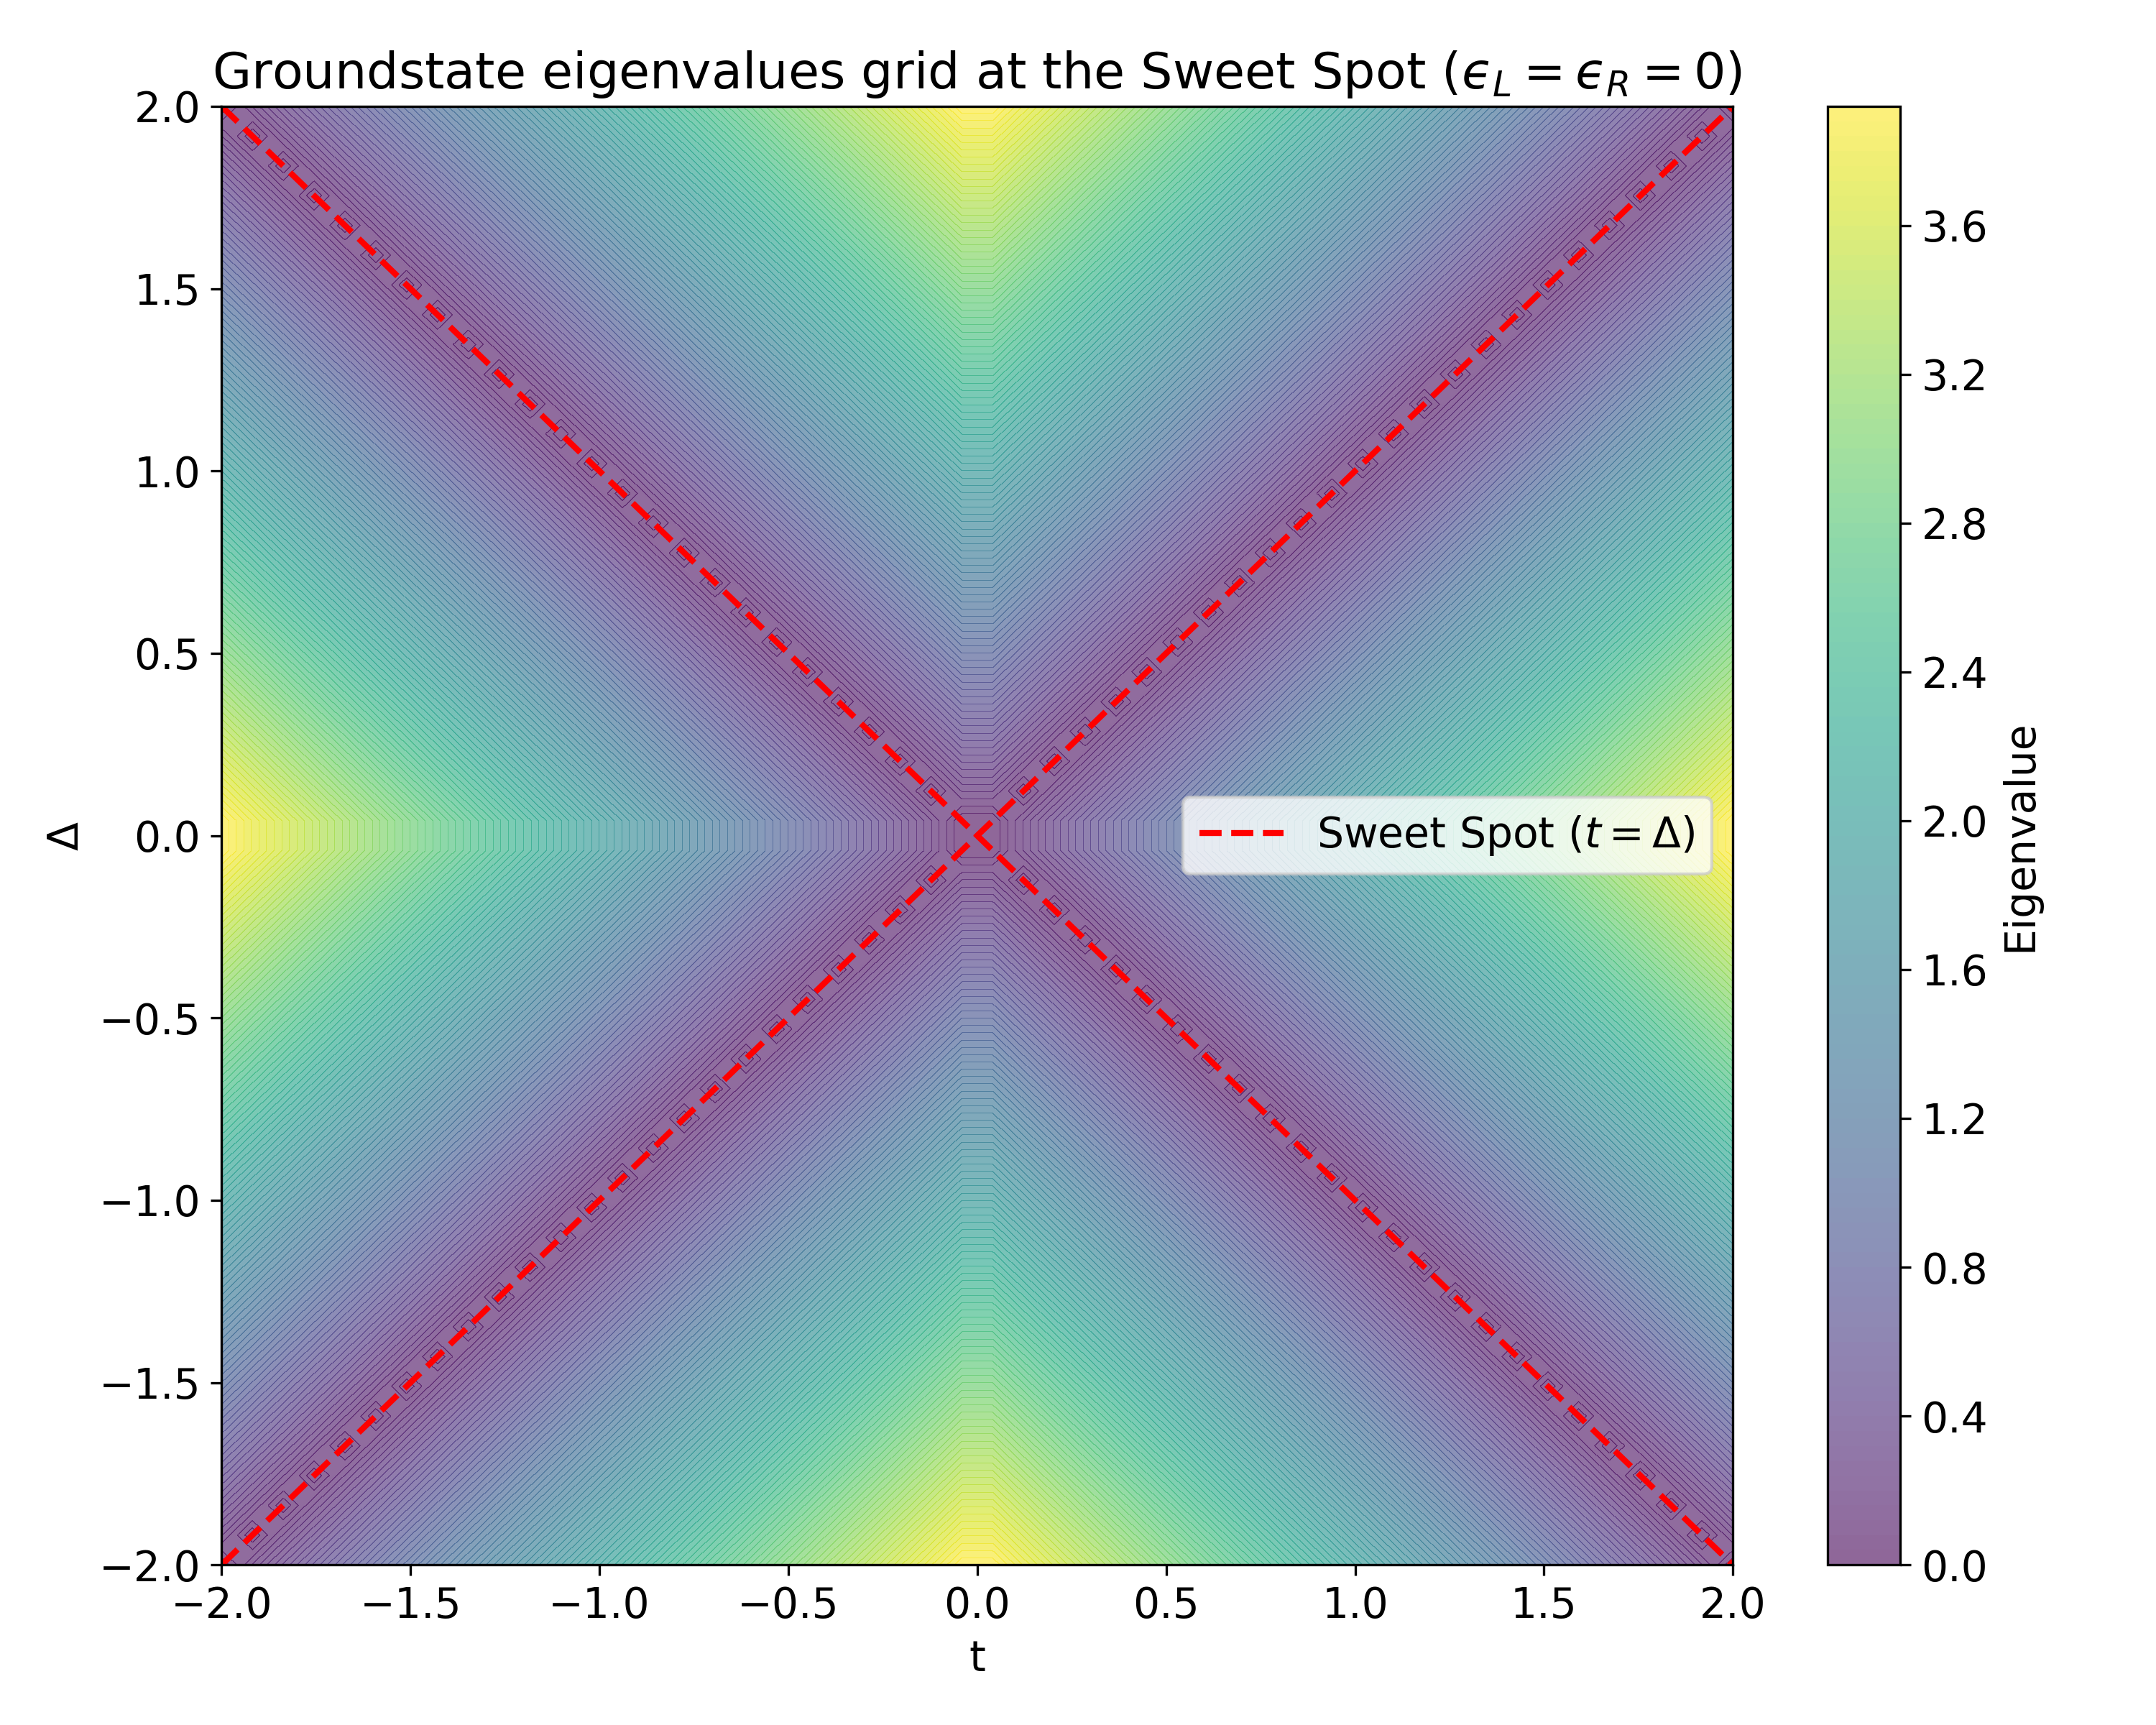
\includegraphics[width=0.7\textwidth]{../Figures/singlebody_sweetspot_grid.png}
  \caption{Contour map of the lowest energy splitting (excited energy eigenvalue minus ground state energy eigenvalue) as a function of $t$ and $\Delta$. The degeneracy is preserved only along the $|t| = |\Delta|$ line (red dashed).}
  \label{fig:sb_grid}
\end{figure}

Additionally, detuning the dot energies $\epsilon_L$ and $\epsilon_R$ while keeping $t = \Delta$ splits the zero-energy states quadratically. This demonstrates that while Poor Man’s Majoranas lack full topological protection, their degeneracy is partially robust against small local perturbations, in agreement with the analytical predictions.
\newpage
\subsection{Many-body model:}
\subsubsection{The Model Hamiltonian:} 
The next step for our model is to proceed from a single-body description to a many-body formalism. This is an essential step, as we need to understand how electron-electron interactions, specifically the Coulomb repulsion $U$, affect the Majorana-like states in the multiple QD–SC–QD system. \par
In order to do so, we need to leave the BdG formalism and work in the many-body basis. This is because the BdG formalism is a mean-field, single-particle approach that cannot capture electron-electron interactions like the Coulomb repulsion $U$. The interaction term we use in order to describe the non-local Coulomb interaction betweem the PMMs is: $H_U=U_{LR}n_Ln_R$, where $n_{α}=d_{α}^{†}d_{α}$ is the number operator for dot $α$.\\
The full Hamiltonian for the QD-SC-QD system with Coulomb interaction is:
$$
H = ∑_{α=L,R} ϵ_{α} d_{α}^{†}d_{α} + t (d_L^{†} d_R + d_R^{†} d_L) + Δ (d_R d_L + d_L^{†} d_R^{†})  + U_{LR} n_L n_R
$$
where $ϵ_{α}$ are the energy levels of the left and right dots, $t$ is the elastic cotunneling amplitude, $Δ$ is the CAR amplitude, and $U_{LR}$ is the non-local Coulomb interaction between electrons on the two dots. The basis states for the two-dot system are: $|0,0⟩$, $|1,0⟩$, $|0,1⟩$, $|1,1⟩$, where $|n_L,n_R⟩$ indicates the occupation of the left and right dots.\par
We can now proceed to construct the Hamiltonian matrix in this many-body basis, where it becomes:
\begin{equation}
H = \begin{pmatrix}
0 & 0 & 0 & Δ \\
0 & ϵ_R & t & 0 \\
0 & t & ϵ_L & 0 \\
Δ & 0 & 0 & ϵ_L + ϵ_R + U_{LR}
\end{pmatrix}
\label{eq:mbHamiltonian}
\end{equation}

\subsubsection{Analytical Work - Exploring the many body Hamiltonian:} 
As mentioned, the many-body Hamiltonian \ref{eq:mbHamiltonian} above is written in the basis order:
$$ |0,0⟩, |0,1⟩, |1,0⟩, |1,1⟩ $$
Due to order and practicality, we can try to rewrite the Hamiltonian in a block-diagonal manner. To do so, we can first investigat the matrix elements we have. The even sector is spanned by the states $|0,0⟩$ and $|1,1⟩$, which correspond to the matrix elements $H_{11}, H_{14}, H_{41}, H_{44}$. The odd sector is spanned by the states $|0,1⟩$ and $|1,0⟩$, which correspond to the matrix elements $H_{22}, H_{23}, H_{32}, H_{33}$.\\
If we reorder the basis as [even, odd] = $[|0,0⟩, |1,1⟩, |0,1⟩, |1,0⟩]$, we obtain:
$$
H = \begin{pmatrix}
0 & Δ & 0 & 0 \\
Δ & ϵ_L + ϵ_R + U_{LR} & 0 & 0 \\
0 & 0 & ϵ_R & t \\
0 & 0 & t & ϵ_L
\end{pmatrix}
$$
This is now block-diagonal, with the even sector in the top-left $2x2$ block and the odd sector in the bottom-right $2x2$ block.\\
In other words, we have:
$$
H = \begin{pmatrix}
H_{even} & 0 \\
0 & H_{odd}
\end{pmatrix}
$$
with:
$$
H_{even} = \begin{pmatrix}
0 & Δ \\
Δ & ϵ_L + ϵ_R + U_{LR}
\end{pmatrix}, \quad
H_{odd} = \begin{pmatrix}
ϵ_R & t \\
t & ϵ_L
\end{pmatrix}
$$
Our next step is to find an expression for the eigenvalues of each sector. For simplicity we will call $S = ϵ_L + ϵ_R + U_{LR}$. Starting with the even sector, we solve the characteristic polynomial:
$$
\text{det}(H_{even} - EI) = \begin{pmatrix}
    -E & Δ \\
    Δ & S - E
\end{pmatrix} =0
$$
This gives us the quadratic equation:
$$
E² - SE + (Δ²) = 0
$$
Using the quadratic formula, we find the eigenvalues for the even sector:
$$E_{even} = \frac{S ± \sqrt{S² + 4Δ²}}{2} = \frac{ϵ_L + ϵ_R + U_{LR} ± \sqrt{(ϵ_L + ϵ_R + U_{LR})² + 4Δ²}}{2}$$
Next, we solve the characteristic polynomial for the odd sector:
$$
\text{det}(H_{odd} - EI) = \begin{pmatrix}
    ϵ_R - E & t \\
    t & ϵ_L - E
\end{pmatrix} =0
$$
This gives us the quadratic equation:
$$(ϵ_R-E)(ϵ_L - E)  - t² = 0$$
$$E² -(ϵ_R-ϵ_L)E + ϵ_R ϵ_L - t² = 0$$
Using the quadratic formula, we find the eigenvalues for the odd sector:
$$E_{odd} = \frac{(ϵ_L + ϵ_R) ± \sqrt{(ϵ_L - ϵ_R)² + 4t²}}{2}$$

\subsubsection{Analytical Work - Finding the Conditions for a Many-body Sweet Spot:}
Now that we have expressions for the eigenvalues of both sectors, we can proceed to find the conditions for a many-body sweet spot. This occurs when the lowest energy eigenvalues of the even and odd sectors are equal:
$$E_{even,min} = E_{odd,min}$$
The first thing to do in order to simplify this problem is to set the dot energies equal to one another, $ϵ_L = ϵ_R = ϵ$, as well as choosing the negative signed square roots. This gives us:
$$E_{even,min} = \frac{2ϵ + U_{LR} - \sqrt{(2ϵ + U_{LR})² + 4Δ²}}{2}$$
$$E_{odd,min} = \frac{2ϵ - \sqrt{4t²}}{2}$$
Setting these equal to one another, we have:
$$\frac{2ϵ + U_{LR} - \sqrt{(2ϵ + U_{LR})² + 4Δ²}}{2} = \frac{2ϵ - 2t}{2}$$
$$U_{LR} - \sqrt{(2ϵ + U_{LR})² + 4Δ²} = -2t$$
Settings $\epsilon= -U/2$ gives:
$$U_{LR} - 2Δ = -2t$$
$$Δ = t + \frac{U_{LR}}{2}$$
So with the parameters $ϵ_L = ϵ_R = -\frac{U_{LR}}{2}$ and $t = Δ - \frac{U_{LR}}{2}$, we have found an analytical expression for the many-body sweet spot. This expression shows how the presence of Coulomb interaction $U_{LR}$ shifts the conditions for achieving Majorana-like degeneracy in the QD–SC–QD system.
\subsubsection{Numerical Simulations - Parameter search for the many-body sweet spot:}
Here, we will start by investigating the parameters needed for the emergence of Majorana-like modes in the many-body Hamiltonian. We will do this by numerically diagonalizing the Hamiltonian matrix in Eq. \ref{eq:mbHamiltonian} for a range of parameters $ϵ_L, ϵ_R, t, Δ, U_{LR}$.\\
In order to determine if we have found a many-body sweet spot, we will calculate the different measurements that we meantioned in section \ref{sec:IdentifyingMajoranaModes}, where we introduced energy degeneracy, local distinguishability, Majorana polarization, and charge expectation values.\\
We will start by exploring how the Coulomb interaction $U_{LR}$ and the tunneling amplitude $t$ effect the emergence of Majorana modes. We will use the analytical expression we found for the first part of the parameter search. We will set the dot energies to $ϵ_L = ϵ_R = -\frac{U_{LR}}{2}$, and set $Δ = t + \frac{U_{LR}}{2}$. We will then vary $U_{LR}$ and $t$ over a reasonable range, and calculate the Majorana metrics for each parameter set.\\
\begin{figure}[htbp]
  \centering
  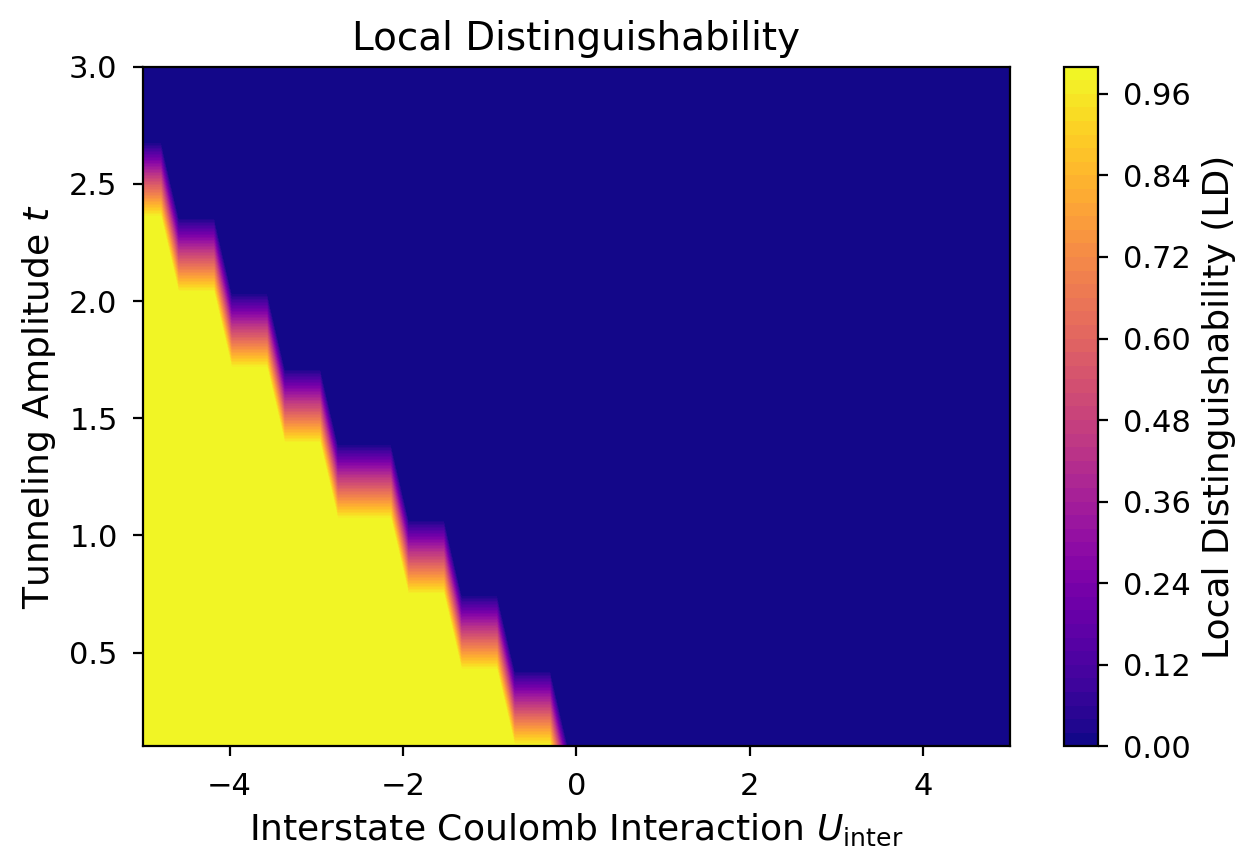
\includegraphics[width=0.7\textwidth]{../Figures/LD_mb.png}
  \caption{Local Distinguishability (LD) as a function of $U_{LR}$ and $t$. The sweet spot region with low (0) LD indicates the presence of Majorana-like modes. We can see that for all positive values of $U_{LR}$, there exists a corresponding $t$ that minimizes LD.}
  \label{fig:mb_LD}
\end{figure}
\begin{figure}[htbp]
  \centering
  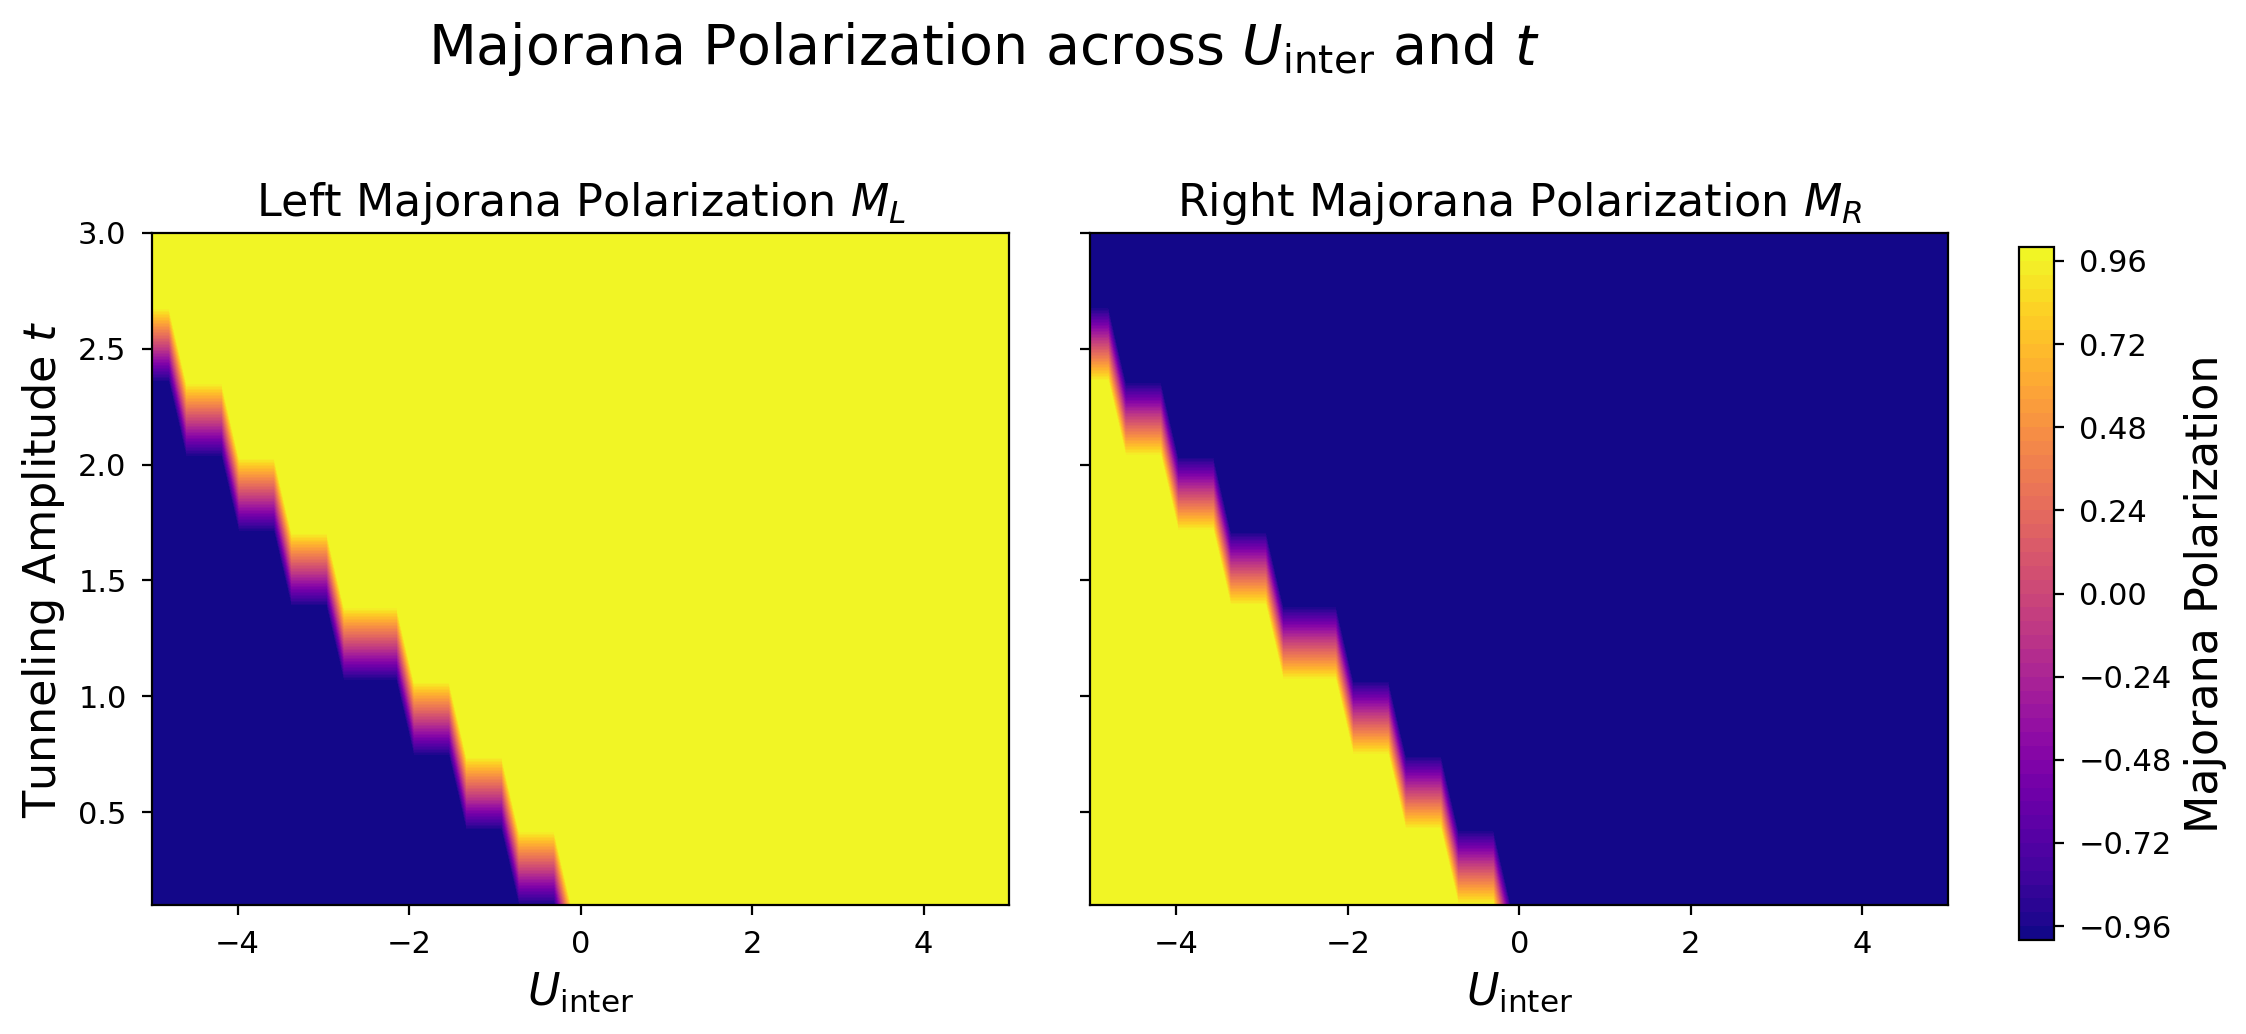
\includegraphics[width=1\textwidth]{../Figures/MP_mb.png}
  \caption{Majorana Polarization (MP) as a function of $U_{LR}$ and $t$. Here we can see that when LD is minimized, MP approaches the ideal values of ±1, confirming the presence of well-localized Majorana-like modes. Also note that where LD is zero, $MP_R=-MP_L$, which is what we expect for Majorana modes.}
  \label{fig:mb_MP}
\end{figure}
Figures ~\ref{fig:mb_LD} and ~\ref{fig:mb_MP} show the results of this parameter search. We can see that there exists a large region for both $t$ and $U_{LR}$ in the parameter space where the local distinguishability (LD) is minimized, indicating that the two ground states are locally indistinguishable. Correspondingly, the Majorana polarization (MP) approaches the ideal values of ±1 in this region, confirming the presence of well-localized Majorana-like modes.
\newpage 
\begin{figure}
  \centering
  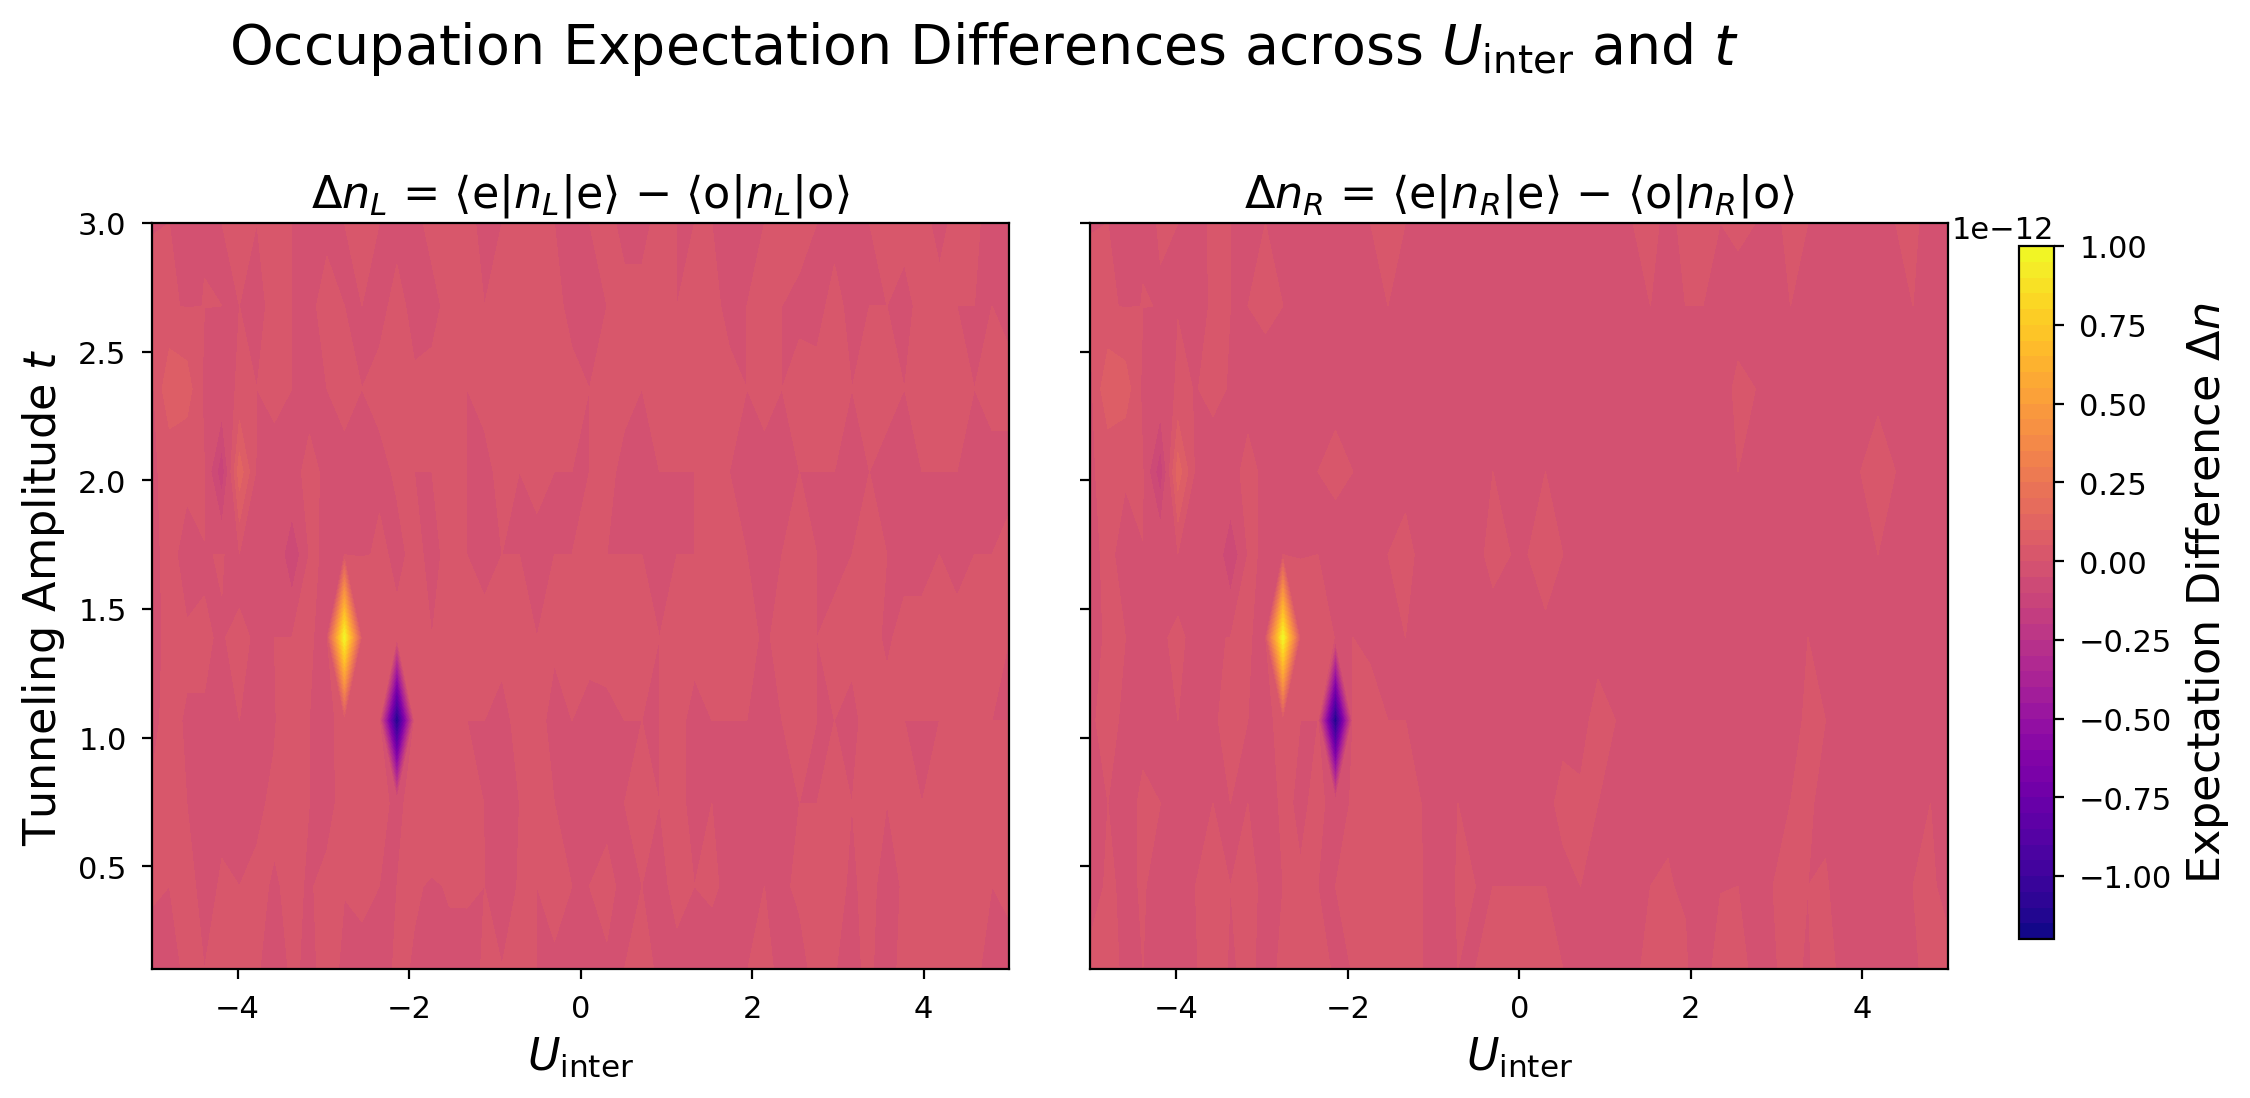
\includegraphics[width=1\textwidth]{../Figures/Exp_mb.png}
  \caption{Charge expectation values $\bra{e}n_{L(R)}\ket{e}$ and $\bra{o}n_{L(R)}\ket{o}$ as a function of $U_{LR}$ and $t$. The charge expectation values for both ground states converge in the sweet spot region, indicating local indistinguishability.}
  \label{fig:mb_charge}
\end{figure}
\begin{figure}
  \centering
  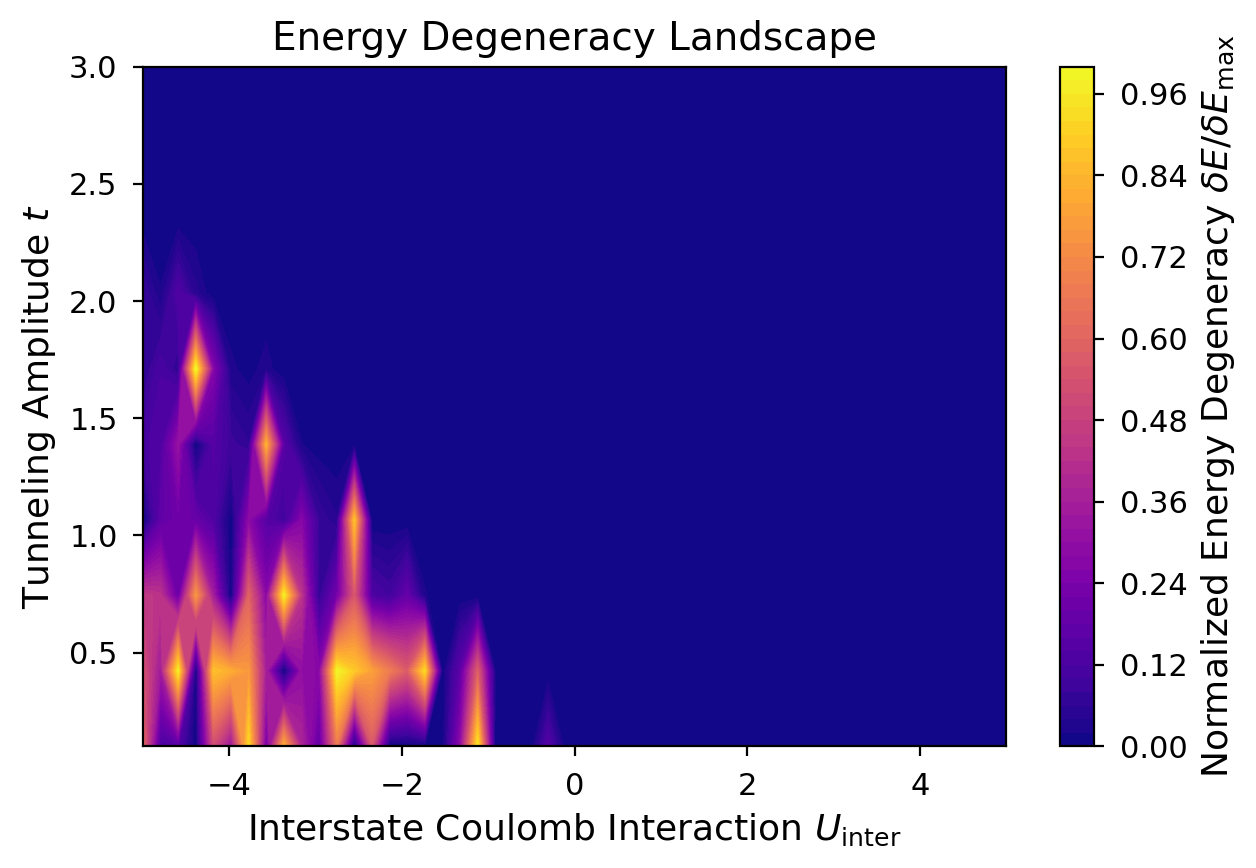
\includegraphics[width=0.7\textwidth]{../Figures/degen_mb.png}
  \caption{Normalized energy splitting $\delta E$ as a function of $U_{LR}$ and $t$. The energy splitting approaches zero in the sweet spot region, confirming the degeneracy of the ground states.}
  \label{fig:mb_deltaE}
\end{figure}
Figures ~\ref{fig:mb_charge} and ~\ref{fig:mb_deltaE} further support the identification of the many-body sweet spot. The charge expectation values for both ground states converge in the sweet spot region, indicating local indistinguishability. Additionally, the normalized energy splitting $\delta E$ approaches zero in this region, confirming the degeneracy of the ground states. Together, these results demonstrate that by tuning $U_{LR}$ and $t$ according to our analytical expression, we can achieve conditions favorable for the emergence of Majorana-like modes in the interacting QD–SC–QD system.
\newpage
In order to further investigate how presise the analytical solutions are, we can take another approach to find the many-body sweet spot. We can do this by fixing $U_{LR}$ and $Δ$, and then varying $ϵ_L, ϵ_R,$ and $t$, and from there we can see if the sweet spots fall in the regions where it was analytically predicted to be.\\
\begin{figure}[htbp]
  \centering
  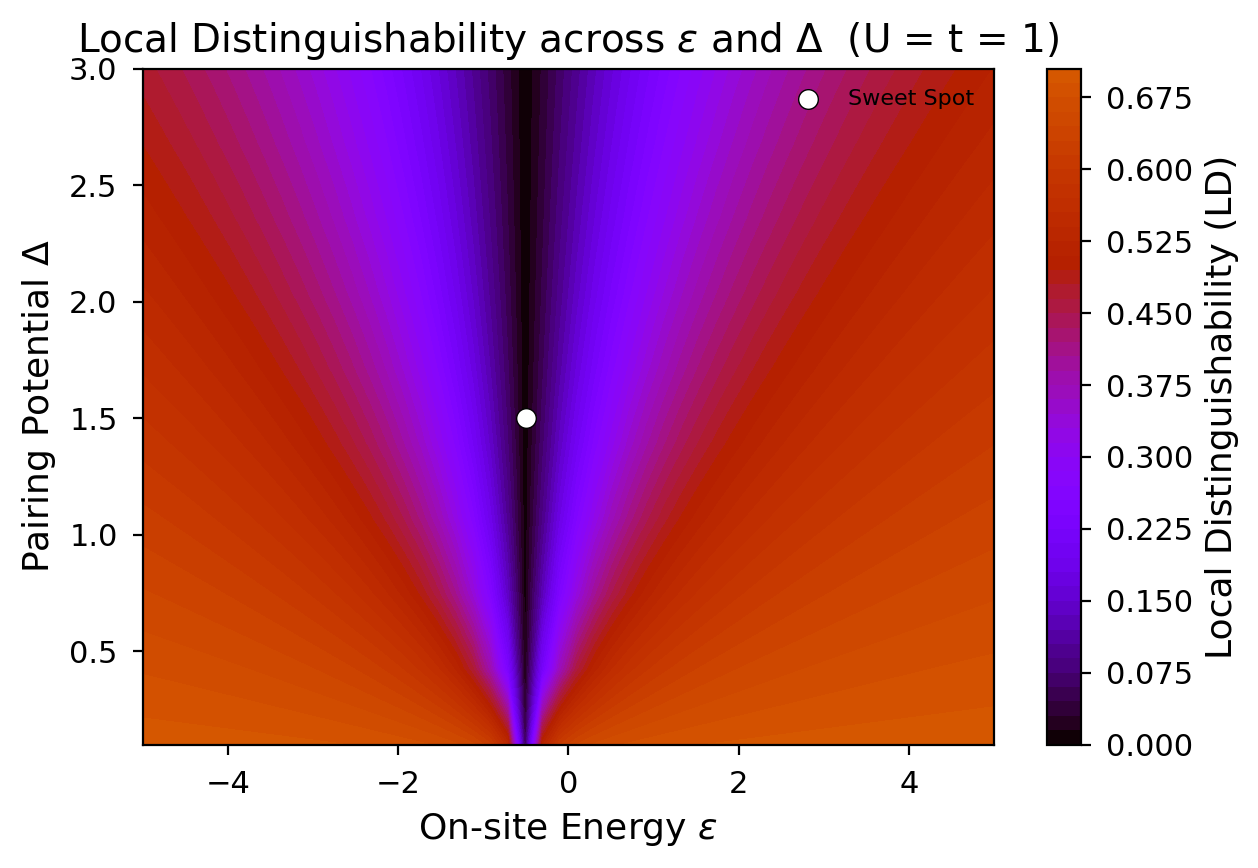
\includegraphics[width=0.7\textwidth]{../Figures/LD_anal.png}
  \caption{Local Distinguishability (LD) as a function of $ϵ_L,ϵ_R$ and $t$ for fixed $U_{LR} = 1$ and $Δ = 1$. The white dot indicates the analytically predicted sweet spot condition. The region of low LD aligns well with the analytical prediction, confirming the presence of Majorana modes.}
  \label{fig:mb_LD_anal}
\end{figure}
\begin{figure}[htbp]
  \centering
  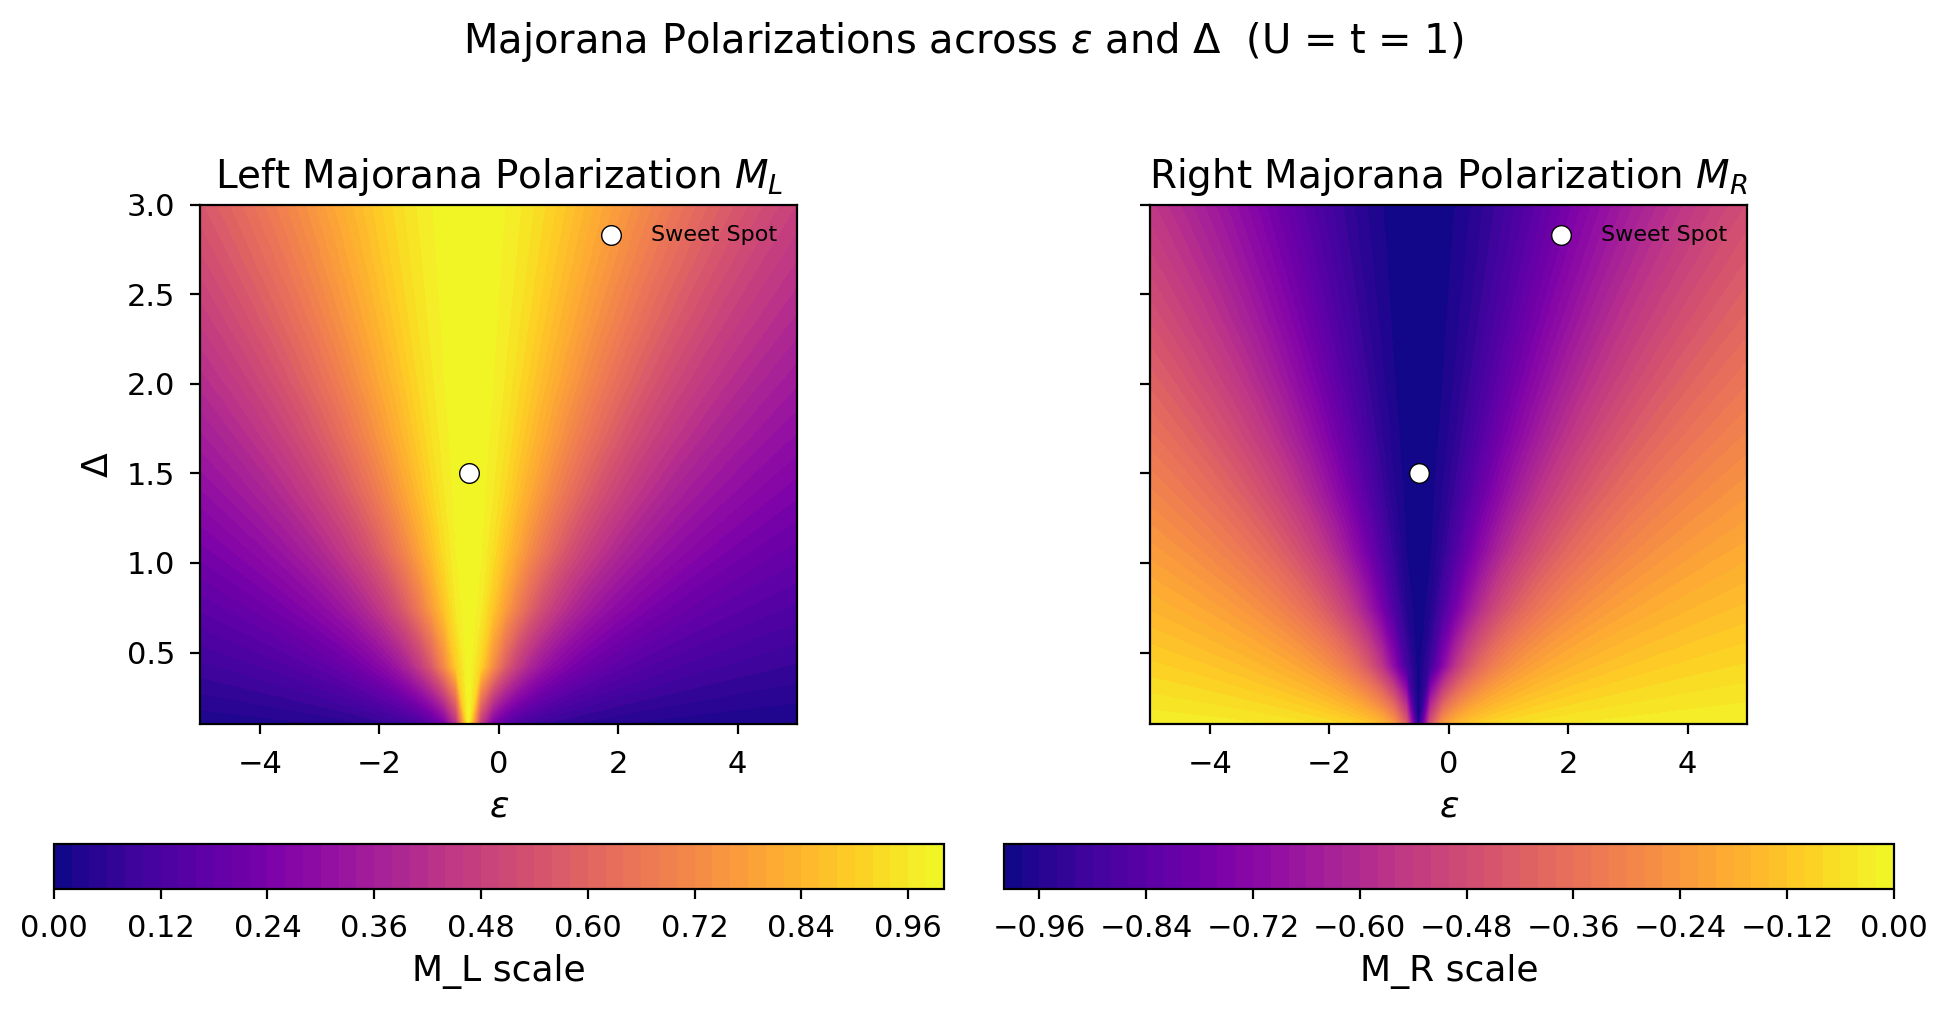
\includegraphics[width=1\textwidth]{../Figures/MP_anal.png}
  \caption{Majorana Polarization (MP) as a function of $ϵ_L,ϵ_R$ and $t$ for fixed $U_{LR} = 1$ and $Δ = 1$. The white dot indicates the analytically predicted sweet spot condition. The MP approaches ±1 at the dot, confirming the presence of Majorana-like modes as predicted analytically.}
  \label{fig:mb_MP_anal}
\end{figure}
Figures ~\ref{fig:mb_LD_anal} and ~\ref{fig:mb_MP_anal} show the results of this alternative parameter search. The white dot indicate the analytically predicted sweet spot condition. We can see that the regions of low local distinguishability (LD) and high Majorana polarization (MP) align well with the analytical predictions, confirming the accuracy of our earlier derived conditions for the emergence of Majorana-like modes in the many-body QD–SC–QD system.
\newpage  
\begin{figure}
  \centering
  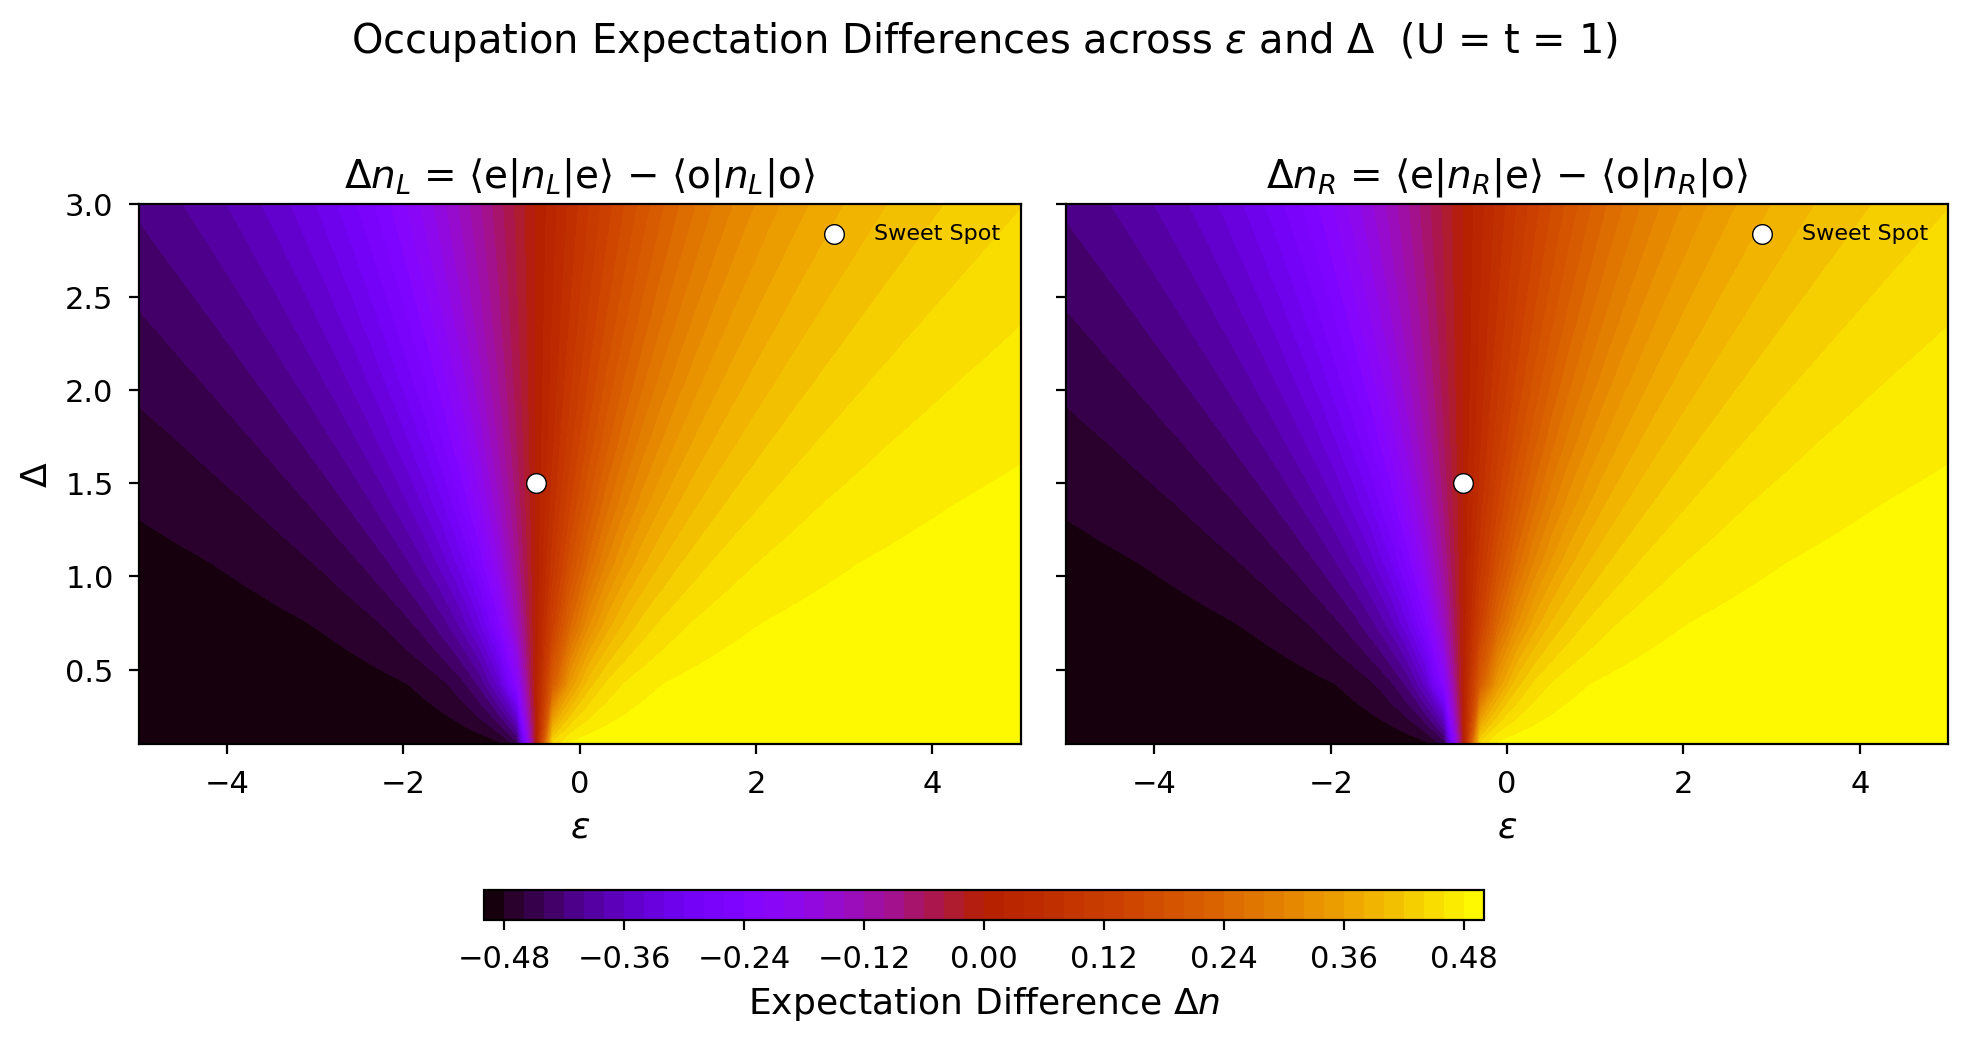
\includegraphics[width=1\textwidth]{../Figures/Exp_anal.png}
  \caption{Charge expectation values $\bra{e}n_{L(R)}\ket{e}$ and $\bra{o}n_{L(R)}\ket{o}$ as a function of $ϵ_L,ϵ_R$ and $t$ for fixed $U_{LR} = 1$ and $Δ = 1$. The white dot indicates the analytically predicted sweet spot condition. The charge expectation values converge at the dot, indicating local indistinguishability as predicted.}
  \label{fig:mb_charge_anal}
\end{figure}
\begin{figure}
  \centering
  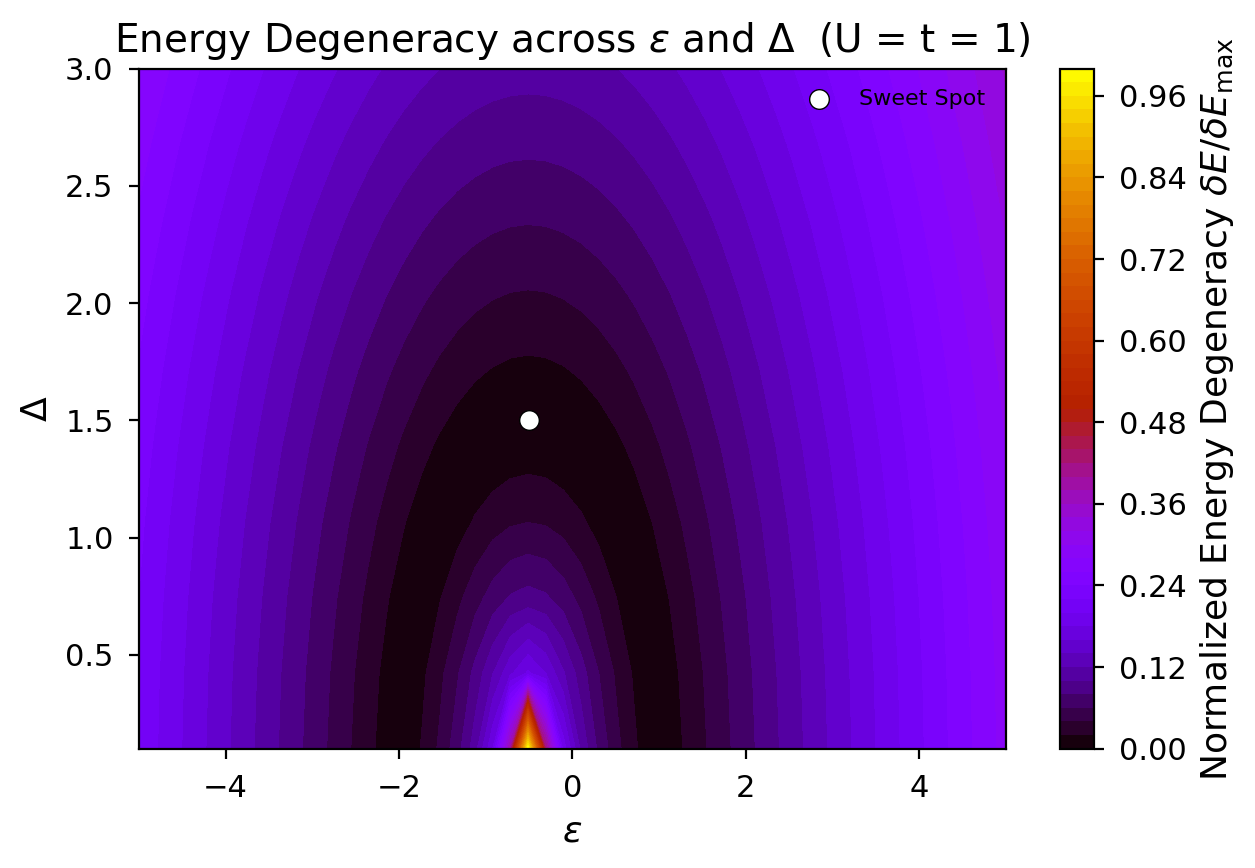
\includegraphics[width=0.7\textwidth]{../Figures/degen_anal.png}
  \caption{Normalized energy splitting $\delta E$ as a function of $ϵ_L,ϵ_R$ and $t$ for fixed $U_{LR} = 1$ and $Δ = 1$. The white dot indicates the analytically predicted sweet spot condition. The energy splitting approaches zero at the dot, confirming the degeneracy of the ground states as predicted.}
  \label{fig:mb_deltaE_anal}
\end{figure}
Figures ~\ref{fig:mb_charge_anal} and ~\ref{fig:mb_deltaE_anal} further validate the analytical predictions. The charge expectation values for both ground states converge at the analytically predicted sweet spot, indicating local indistinguishability. Additionally, the normalized energy splitting $\delta E$ approaches zero at this point, confirming the degeneracy of the ground states.\\
By collectively looking at where the different metrics indicate the presence of Majorana-like modes, we can see how the position of the sweet spot aligns with each individual metric. This summarizes how the analytically predicted sweet spot conditions hold up against the numerical simulations.
\newpage

\section{Discussion and Conclusion}
\subsection{Synthesize my Findings:} Summarize what we learned from the calculations. " The analysis confirmed that zero-energy Majorana modes emerge under fine-tuned conditions... Numerical simulations revealed that this degeneracy is fragile and splits when deviating from the sweet spot, quantifying the limited protection of PMMs."\par
\subsection{Connect to Broader Context:} Briefly discuss how the properties you explored (the energy splitting, wavefunction overlap) would affect potential braiding operations (note section 5.2.3) and what this means for using PMMs in quantum computing.\par
\subsection{Future Directions:} Suggest next steps for a full thesis. This include modeling disorder, investigating longer chains (three or more dots), or numerically simulate braiding protocol.

\newpage
\section{Appendix}
\subsection{Explanations}

\textbf{Cooper pairs}: Pairs of electrons bound together at low temperatures in a superconductor, leading to superconductivity.

\textbf{p-wave superconductivity}: A type of superconductivity where the Cooper pairs have angular momentum \(l=1\), leading to odd-parity pairing.  

\textbf{s-wave superconductivity}: Conventional superconductivity where Cooper pairs have zero angular momentum (\(l=0\)) and even-parity pairing.  

\textbf{Zeeman effect}: The splitting of energy levels in a magnetic field due to the interaction of the field with electron spins.  

\textbf{Coulomb interaction}: The repulsive interaction between electrons due to their electric charge, often represented as an on-site energy \(U\) in quantum dot systems.



\end{document}











